\chapter{RESULTADOS ALOMÉTRICOS E MORFOMÉTRICOS}\label{sec:resultados-alometricos-morfometricos}

Nesta seção apresenta-se os resultados alométricos e morfométricos obtidos com os modelos gerados pelos Algoritmos~\ref{algo:CCOVenosoArterial},~\ref{algo:FlorestaDeArvoresComInvasao} e~\ref{algo:COAT}.
O Algoritmo~\ref{algo:CCOVenosoArterial} foi implementado na linguagem de programação C por 
Queiroz~\cite{Queiroz2013}. Os demais algoritmos propostos foram implementados na linguagem 
de programação C++. 
A visualização dos modelos gerados nas simulações foi realizada usando o programa de visualização científica 
ParaView~\cite{Ayachit2015} (versão 5.8.1).
O computador usado para executar as simulações dos algoritmos tem processador Intel Pentium G4560 (dual core 
de 3,5 GHz), memória RAM DDR4 de 8 GB e sistema operacional Ubuntu 22.04.

\section{ÁRVORES ARTERIAIS E VENOSAS ACOPLADAS}\label{sec:resultados-arvores-acopladas}

Como estudo de caso, um exemplo da aplicação do Algoritmo~\ref{algo:CCOVenosoArterial} é apresentado  
para a criação de um modelo do sistema vascular arteriovenoso renal que é formado por duas árvores. 
Na Tabela~\ref{tab:parametros-modelo-rim} tem-se os parâmetros utilizados nas simulações, 
que estão de acordo com \cite{Kretowski2004} em relação às condi\c{c}\~oes de contorno de pressão.
A posição proximal do segmento raiz de cada árvore do sistema renal foi aqui 
determinada a partir da rede vascular do atlas digital Anatomium$^{\text{TM}}$~\cite{Langenkamp2015} 
e da localização dos ramos principais de cada árvore mostrada em \cite{Kretowski2004}.
A superfície do domínio de perfusão representando o rim também foi determinada a partir do mesmo atlas.

\begin{table}[!htb]
\centering
\captiondelim{: }
\caption{Parâmetros utilizados para a gera\c{c}\~ao do sistema vascular renal.}
 \begin{tabular}{|c|cc|}
\hline
Parâmetro             &Árvore arterial & Árvore venosa\\
\hline
   $p^t_{perf}$ (mmHg) & 95 & 10 \\
   $p^t_{term}$ (mmHg) & 15 & 5 \\
\hline
   $Q^t_{perf}$ (mL/min) & \multicolumn{2}{|c|}{617,5}\\
$Q^t_{term}$ (mL/min) & \multicolumn{2}{|c|}{0,19297}\\
 $N_{term}$ & \multicolumn{2}{|c|}{3200}\\
$D_{perf}$  (cm$^3$) & \multicolumn{2}{|c|}{57,01} \\
$\gamma$  & \multicolumn{2}{|c|}{2,2} \\
\hline
\end{tabular}
\fonte{Queiroz (2018).}
\label{tab:parametros-modelo-rim}
\end{table}

Na Figura~\ref{fig:resRim3DAcopla} são exibidas as árvores vasculares geradas para 
um domínio representando o rim utilizando o  
Algoritmo~\ref{algo:CCOVenosoArterial}. Destaca-se nesta figura que as árvores 
não estão distribuídas espacialmente de modo uniforme no domínio representando 
o rim humano, isto ocorre por não ter sido utilizado uma distribuição uniforme de 
pontos terminais dentro deste domínio. Isto é compatível com a anatomia deste 
órgão, pois sua vascularização tende a se localizar na sua parênquima, 
ou seja, na região funcional do volume ocupado pela superfície 
envolvente do órgão, que no caso do rim se encontra sobre a região periférica do seu volume.

\begin{figure}[!htb]
  \centering
  \captiondelim{: }
  \caption{Sistema vascular renal gerado.}
  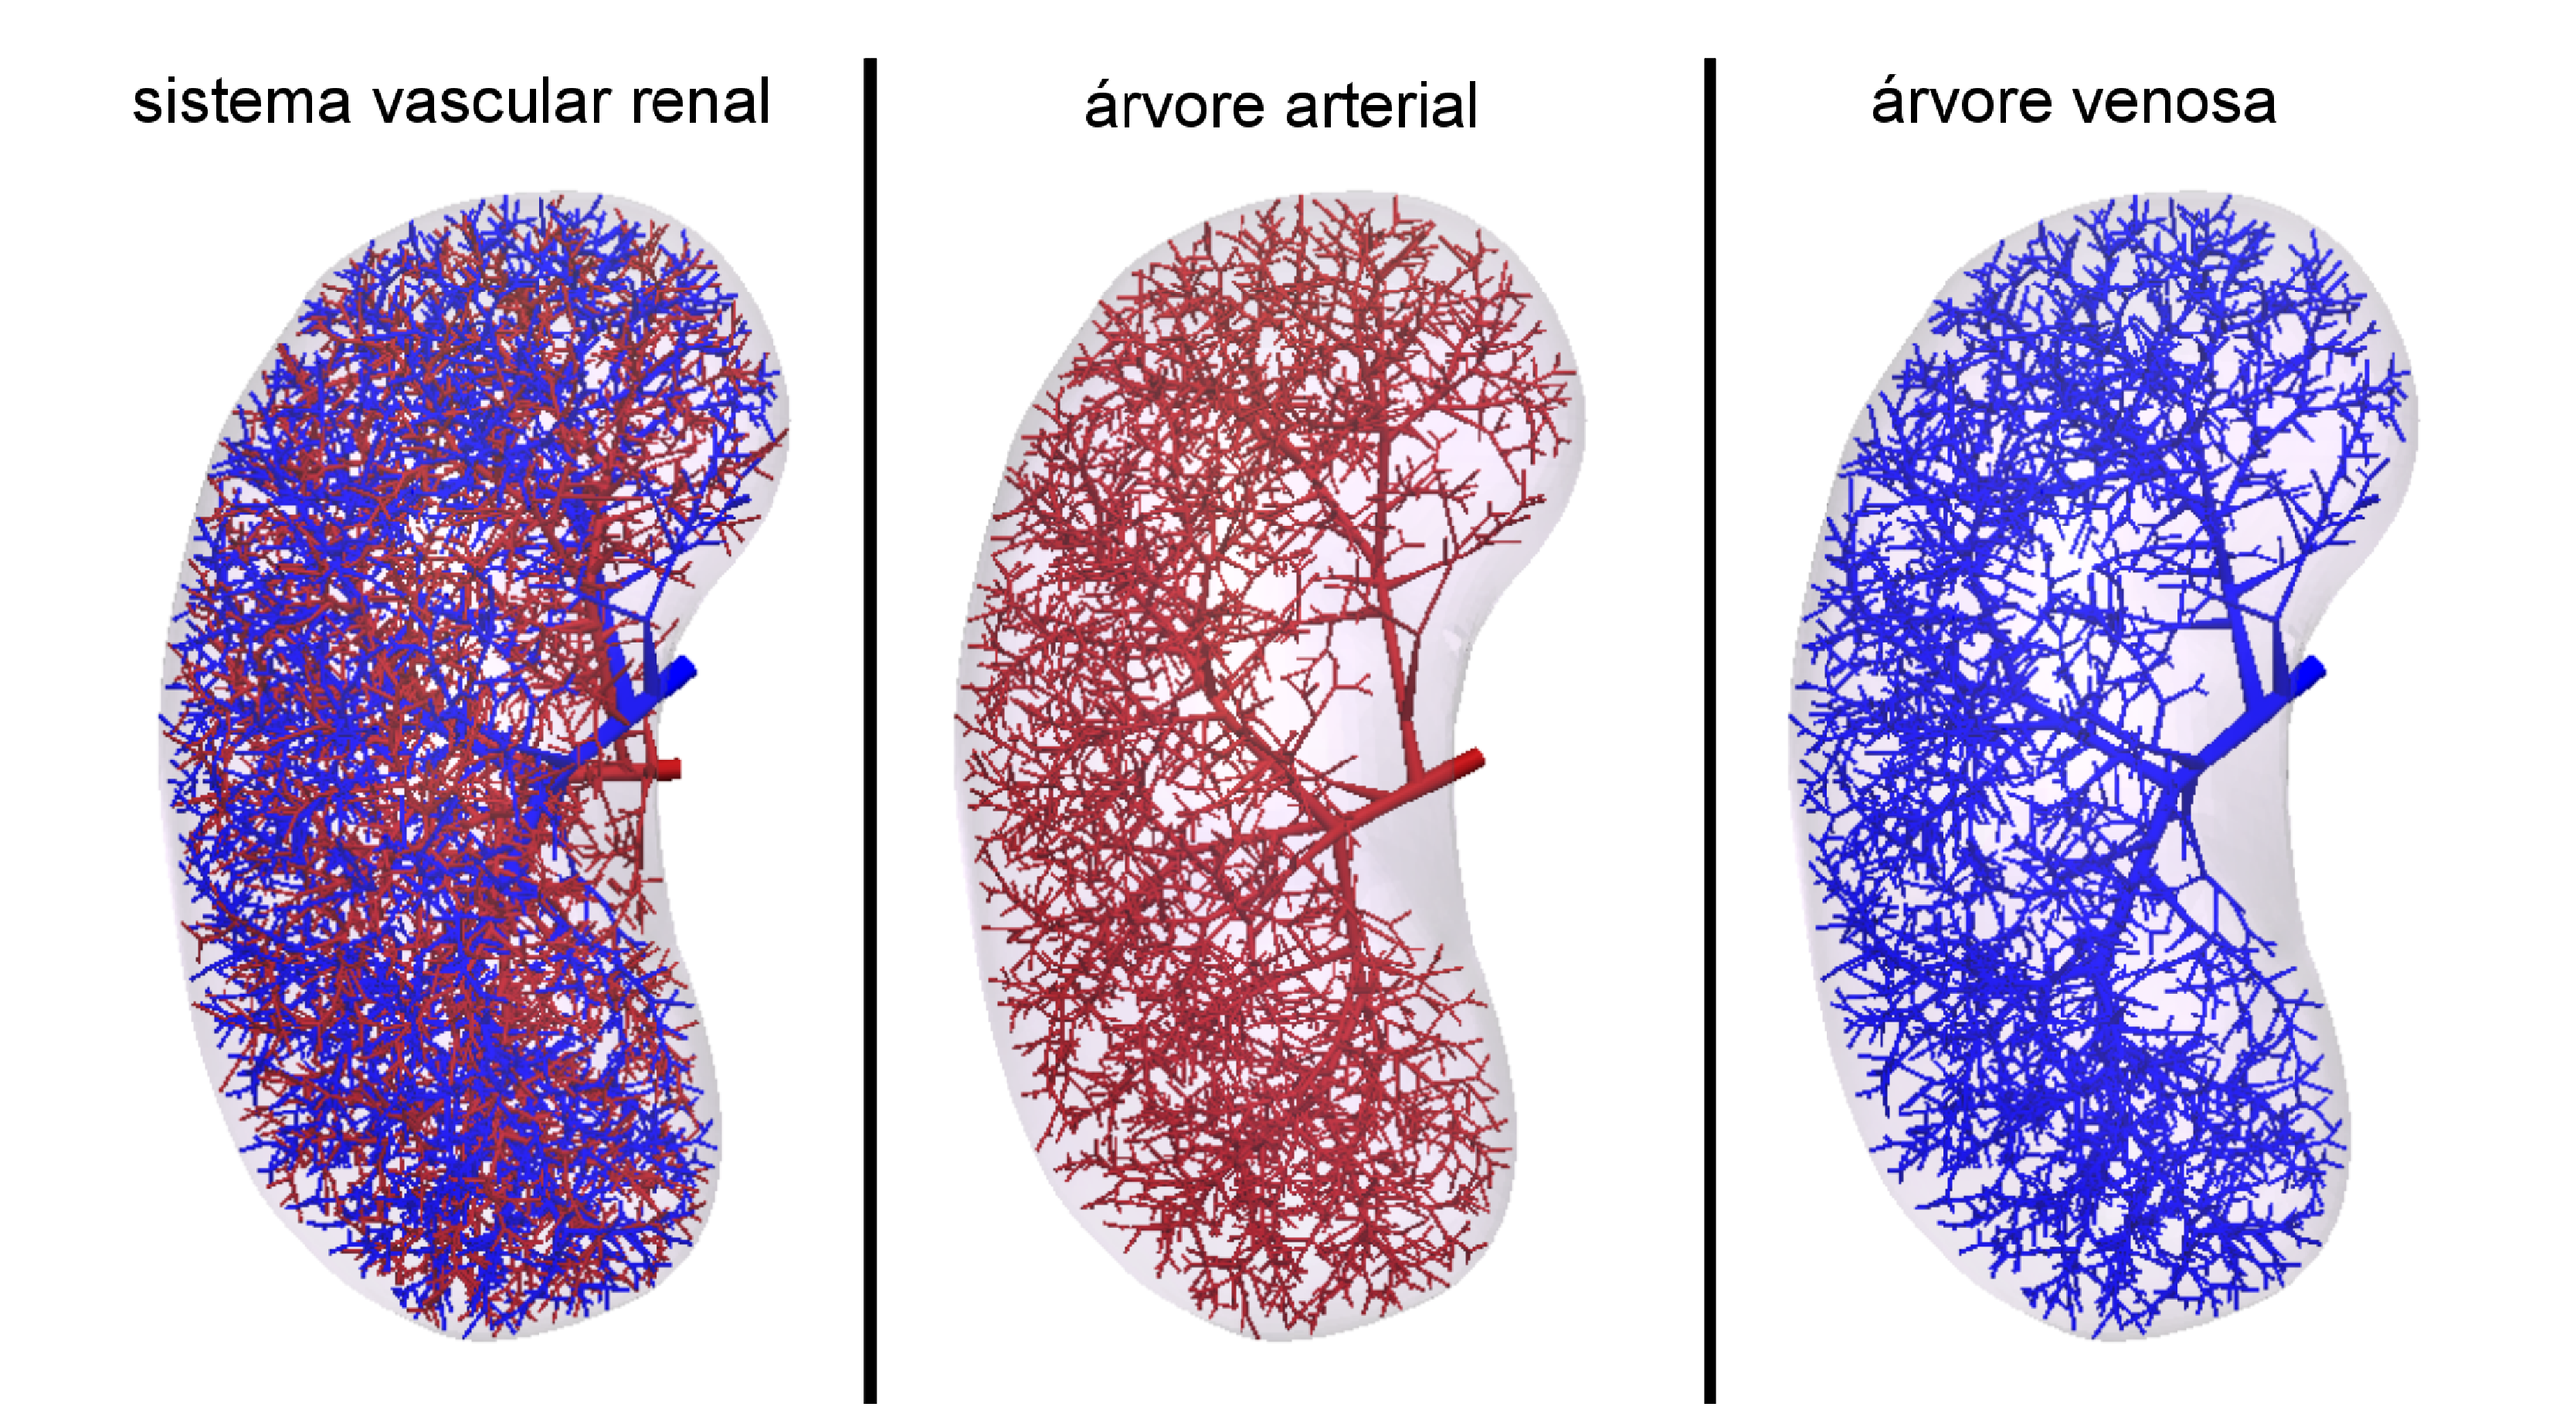
\includegraphics[width=\textwidth]{figuras/modelos-computacionais-de-arvores-circulatorias/DomFix_RimAcoplamentoNaoUniforme.eps}
  \fonte{Queiroz (2018).}
  \label{fig:resRim3DAcopla}
\end{figure}

Na Tabela~\ref{tab:dados-morfometricos-rim}, os resultados morfométricos das árvores arterial e venosa são apresentados. 
Nessa tabela, AA denota a árvore arterial e AV a árvore venosa. A média e o desvio padrão dos resultados 
foram calculados, pois foram gerados 10 modelos do sistema, alterando-se a distribuição dos pontos terminais no 
domínio. Nota-se que o raio do segmento raiz ($r_{iroot}$) do modelo de árvore arterial está consistente com o 
raio de uma artéria renal real, que está entre 2mm e 6mm de acordo com~\cite{Weld2005}. O valor do raio do 
segmento raiz do modelo de árvore venosa está relativamente próximo do valor do raio de uma veia 
renal real, que varia entre 5mm e 7mm conforme~\cite{Satyapal2019}. Como esperado, o raio do segmento raiz 
e o volume intravascular ($V$) são maiores para as árvores venosas do que aqueles das árvores arteriais.

É apresentado ainda na Tabela~\ref{tab:dados-morfometricos-rim} o número 
máximo de níveis de bifurcação ($n_{\max}$), isto é, o número máximo de 
pontos de bifurcação partindo do segmento raiz até o segmento terminal mais distante
na árvore. A Figura~\ref{fig:nivel-de-bifurcacao} ilustra o cálculo do nível de bifurcação
em uma árvore genérica.

\begin{figure}[!htb]
  \centering
  \captiondelim{: }
  \caption{Exemplo do cálculo do nível de bifurcação.}
  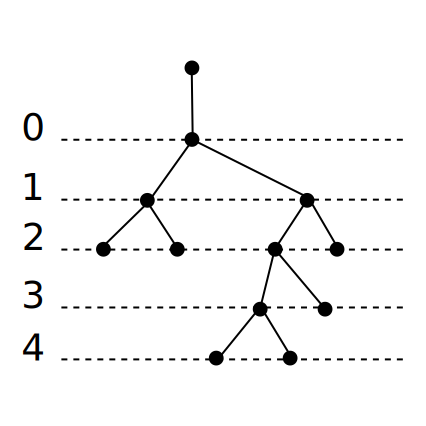
\includegraphics[width=0.25\textwidth]{figuras/modelos-computacionais-de-arvores-circulatorias/nivel-de-bifurcacao.pdf}
  \fonte{Queiroz (2018).}
  \label{fig:nivel-de-bifurcacao}
\end{figure}

\begin{table}[!htb]
\centering
\captiondelim{: }
\caption{Propriedades morfométricas do sistema vascular renal gerado.}
\begin{tabular}{|c|c|c|c|c|c|}
  \hline 
 Árv.  & $r_{iroot}$ (mm) & $r_{\min}$ (mm) & $V$ (mm$^3$) & $n_{\max}$ \\
\hline
AA & $2,0900 \pm 0,0019$ & $0,0138 \pm 0,0017$ & $720,0206 \pm  6,6782 $ & $44 \pm 2$ \\
AV & $4,0862 \pm 0,0106$ & $0,0289 \pm 0,0031$ & $2797,5518 \pm 23,1052$ & $48 \pm 4$ \\
\hline
\end{tabular}
  \fonte{Queiroz (2018).}
\label{tab:dados-morfometricos-rim}
\end{table}

Na Figura~\ref{fig:CurveMorfometricaRim} são apresentadas as curvas morfométricas que relacionam o diâmetro médio 
do segmento em função de seu nível de bifurcação das árvores arterial 
e venosa do sistema renal gerado pelo Algoritmo~\ref{algo:CCOVenosoArterial}. 
Salienta-se que o decaimento apresentado nas curvas se assemelha 
aos dados experimentais oriundos de corrosão vascular de árvores coronarianas reais~\cite{Zamir1987}.

\begin{figure}[!htb]
  \centering
  \captiondelim{: }
  \caption{Curvas morfométricas que relacionam o diâmetro médio do segmento com seu nível de bifurca\c{c}\~ao
das árvores arterial e venosa do sistema renal.) (a) Árvore arterial. (b) Árvore venosa.}
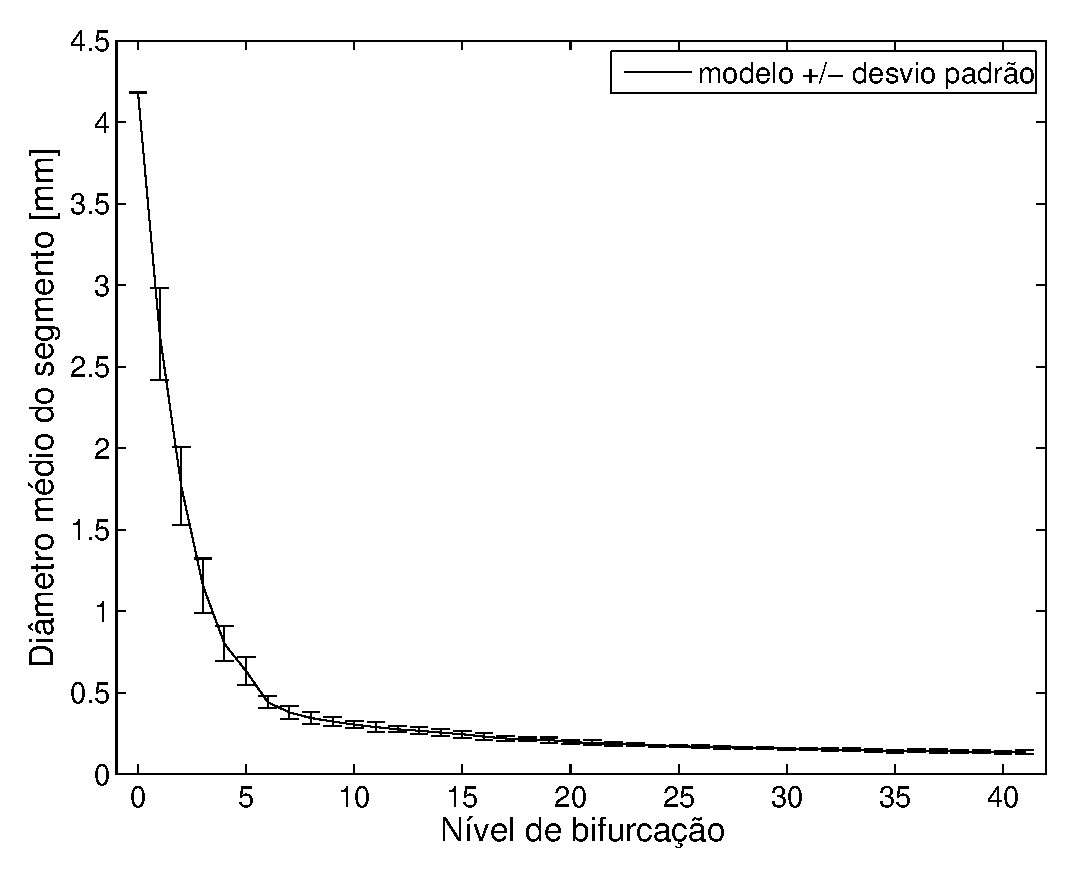
\includegraphics[width=0.49\textwidth]{figuras/modelos-computacionais-de-arvores-circulatorias/res_domfix_nonunif_tree1.eps}
\includegraphics[width=0.49\textwidth]{figuras/modelos-computacionais-de-arvores-circulatorias/res_domfix_nonunif_tree2.eps}

  (a) \hspace{0.5\textwidth} (b)
  \fonte{Queiroz (2018).}
  \label{fig:CurveMorfometricaRim}
\end{figure}

\clearpage

\section{FLORESTAS DE ÁRVORES ARTERIAIS COM COEFICIENTE DE INVASÃO}\label{sec:floresta-invasao-resultados}

Como prova de conceito do Algoritmo~\ref{algo:FlorestaDeArvoresComInvasao}, 
ele foi aplicado em dois domínios de perfusão, sendo um deles bidimensional 
não convexo e o outro tridimensional convexo. O domínio bidimensional não
convexo tem formato de disco, com raio externo de 5 cm e interno de 1,5 cm. 
Já o domínio tridimensional convexo, tem o formato de esfera com raio de 
aproximadamente 2,879 cm (ou seja, para um volume de 100 cm$^3$). Esses 
domínios foram escolhidos de modo a representar a floresta suprindo 
100 $g$ de tecido do miocárdio durante máxima vasodilatação~\cite{Schreiner1993b}.
A Tabela~\ref{tab:parametros-floresta-invasao-2d} apresenta os parâmetros 
usados na execução.

As coordenadas dos pontos 
nesses domínios foram criadas usando o gerador de números aleatórios
dSFMT~\cite{Saito2009}. Ambos os domínios foram ocupados por uma 
floresta com duas árvores ($N_{trees} = 2$) e número total de terminais
igual a 250 ($N_{term} = 250$).
Além disso, os fluxos alvos $q_{targ}^1$ e $q_{targ}^2$, 
respectivamente, referentes às árvores $t = 1$ e $t = 2$, variaram 
conforme indicado na Tabela~\ref{tab:casos-fluxo-duas-arvores}, de tal modo 
que $\dfrac{q_{targ}^1}{q_{targ}^2} = n$, com $n = 1$, 2, \ldots, 10.

No caso do domínio tridimensional (3D), também foram realizados experimentos 
com três árvores ($N_{trees} = 3$), número total de terminais igual a 250 
($N_{term} = 250$) e com fluxos alvos $q_{targ}^1$, $q_{targ}^2$ e $q_{targ}^3$, 
respectivamente, referentes às árvores $t = 1$, $t = 2$ e $t = 3$, variando
conforme indicado na Tabela~\ref{tab:casos-fluxo-tres-arvores}, 
de tal modo que 
$\left(\dfrac{q_{targ}^1}{q_{targ}^2},\, \dfrac{q_{targ}^2}{q_{targ}^3}\right) = (m,\,n)$, 
com $(m,\, n) \in \{1,\, 2,\, 3\}\times \{1,\, 2,\, 3\}$.

Cada um dos casos 
nas Tabelas~\ref{tab:casos-fluxo-duas-arvores} e~\ref{tab:casos-fluxo-tres-arvores} 
foi executado dez vezes, alterando a semente do gerador de números aleatórios em cada execução.

\begin{table}[!htb]
  \centering \captiondelim{: }
  \caption{
    Casos para a distribuição dos fluxos alvos $q_{targ}^1$ e $q_{targ}^2$,
    respectivamente, referentes às árvores $t = 1$ e $t = 2$.
  }
  \begin{tabular}{|c|c|c|c|}
    \hline
    Caso & $q_{targ}^1$ (\%) & $q_{targ}^2$ (\%) \\ \hline
    1 & 50,00 & 50,00 \\ \hline
    2 & 66,70 & 33,30 \\ \hline
    3 & 75,00 & 25,00 \\ \hline
    4 & 80,00 & 20,00 \\ \hline
    5 & 83,40 & 16,60 \\ \hline
    6 & 85,70 & 14,30 \\ \hline
    7 & 87,50 & 12,50 \\ \hline
    8 & 88,90 & 11,10 \\ \hline
    9 & 90,00 & 10,00 \\ \hline
    10 & 90,90 & 9,10\\ \hline
  \end{tabular}
  \fonteAutor{2022}\label{tab:casos-fluxo-duas-arvores}
\end{table}

\begin{table}[!htb]
  \centering \captiondelim{: }
  \caption{
    Casos para a distribuição dos fluxos alvos $q_{targ}^1$, $q_{targ}^2$ e 
    $q_{targ}^3$, respectivamente, referentes às árvores $t = 1$, $t = 2$ e 
    $t = 3$.
  }
  \begin{tabular}{|c|c|c|c|c|}
    \hline
    Caso & $q_{targ}^1$ (\%) & $q_{targ}^2$ (\%) & $q_{targ}^3$ (\%) \\ \hline
    1 & 33,40 & 33,30 & 33,30 \\ \hline
    2 & 40,00 & 40,00 & 20,00 \\ \hline
    3 & 42,90 & 42,70 & 14,40 \\ \hline
    4 & 50,00 & 25,00 & 25,00 \\ \hline
    5 & 57,20 & 28,50 & 14,30 \\ \hline
    6 & 60,00 & 30,00 & 10,00 \\ \hline
    7 & 60,00 & 20,00 & 20,00 \\ \hline
    8 & 66,70 & 22,20 & 11,10 \\ \hline
    9 & 69,20 & 23,10 & 7,70 \\ \hline
  \end{tabular}
  \fonteAutor{2022}\label{tab:casos-fluxo-tres-arvores}
\end{table}

\begin{table}[!htb]
 \centering
 \captiondelim{: }
 \caption{
   Parâmetros usados no Algoritmo~\ref{algo:FlorestaDeArvoresComInvasao}
   em conformidade com os dados da literatura~\cite{Jaquet2019,Karch1999,Schreiner1993b}.}
 \begin{tabular}{|l|l|}
  \hline
  Parâmetro & Valor \\ \hline
  Viscosidade ($\mu$) & $3,6\cdot 10^{-3}$ Pa \\ \hline
  Fluxo de perfusão ($Q_{perf}$) & $8,33$ cm$^3$/s \\ \hline        
  Pressão de perfusão ($p_{perf}$) & $1,333 \cdot 10^4$ Pa ($\approx 100$ mmHg)\\ \hline
  Pressão terminal ($p_{term}$) & 
  \begin{tabular}{c}
    Caso 2D: $8,399 \cdot 10^3$ Pa ($\approx 63$ mmHg). \\
    Caso 3D: $9,599\cdot 10^3$ Pa ($\approx 72$ mmHg).
  \end{tabular}\\\hline
  Expoente de bifurcação ($\gamma$) & 3,0 \\ \hline
  Número de árvores ($N_{trees}$) & 2 \\ \hline
  Número de terminais ($N_{term}$) & 250 \\ \hline
  Número de segmentos vizinhos ($N_{con}$) & 20 \\ \hline
  Coeficiente de invasão ($\alpha$) & 0,75 \\ \hline
  Número de tentativas ($N_{toss}$) & 10 \\ \hline
  Fator de redução ($\beta$) & 0,9 \\ \hline
 \end{tabular}
 \fonteAutor{2022}
 \label{tab:parametros-floresta-invasao-2d}
\end{table}

\clearpage

Os resultados obtidos na execução dos casos estão descritos 
nas Seções~\ref{sec:floresta-com-invasao-caso-2d},
\ ~\ref{sec:floresta-com-invasao-caso-3d} e~\ref{sec:floresta-com-invasao-caso-3arvores-3d}. 
Para analisar o território $T_t$ ocupado pela árvore $t$, 
empregou-se o diagrama de Voronoi usando os pontos $P_i$ 
distais dos segmentos de $t$, conforme~\eqref{def:diagrama-voronoi}. 

Em~\cite{West1997} é apresentado que a massa $M$ da aorta de mamíferos 
e a área $Y$ de sua seção transversal estão relacionadas por uma lei alométrica no
formato:
\begin{equation}
  Y = Y_0 M^\frac{3}{4},
  \label{eq:lei-alometrica-secao-transversal-vs-area}
\end{equation}
onde $Y_0$ é uma constante. Considerando que o raio do segmento raiz de cada árvore $t$ 
seja $r_{iroot,\,t}$ e que o respectivo território ocupado por essa árvore seja $T_t$, 
deseja-se investigar se eles estão relacionados através de alguma lei 
como~\eqref{eq:lei-alometrica-secao-transversal-vs-area}. 

Supondo que as árvores $i$ e $j$ de uma floresta são tais 
que $\dfrac{T_i}{T_j} \neq 1$, deseja-se analisar a existência de um expoente
$b$ tal que:
\begin{eqnarray}
  \begin{cases}
    \pi r_{iroot,\,i}^2 = Y_0T_i^{b}\\
    \pi r_{iroot,\,j}^2 = Y_0T_j^{b}
  \end{cases}\implies
  \dfrac{r_{iroot,\,i}^2}{r_{iroot\,j}^2} = \dfrac{T_i^{b}}{T_j^{b}}
  \implies
  \dfrac{\ln\left(\dfrac{r_{iroot,\,i}}{r_{iroot,\,j}}\right)}{\ln\left(\dfrac{T_i}{T_j}\right)} = \dfrac{b}{2}
  \label{eq:desenvolvimento-lei-alometrica}
\end{eqnarray}

Nota-se que a restrição $\dfrac{T_i}{T_j} \neq 1$ deve ser utilizada 
para que  $\ln\left(\dfrac{T_i}{T_j}\right) \neq 0$ e assim não ocorra uma divisão 
por zero em~\eqref{eq:desenvolvimento-lei-alometrica}. Por praticidade na 
análise dos resultados, nesse trabalho adota-se a convenção:
\begin{equation}
  \delta_{i, j} = \dfrac{\ln\left(\dfrac{r_{iroot,\,i}}{r_{iroot,\,j}}\right)}{\ln\left(\dfrac{T_i}{T_j}\right)}
  \label{eq:lei-alometrica-delta-ij}
\end{equation}

\clearpage

\subsection{Caso bidimensional}\label{sec:floresta-com-invasao-caso-2d}

A Tabela~\ref{tab:resultados-floresta-com-invasao-2d} resume os resultados
das simulações para verificar o fluxo obtido e o território ocupado, em contraste com o 
fluxo alvo fornecido.
Verifica-se que o erro relativo médio entre o fluxo obtido e o fluxo alvo foi 
de $0,018 \pm 0,024$. Isso representa um erro inferior a $2\%$. 
Além disso, a relação entre o fluxo obtido e o território ocupado estão correlacionados com um
coeficiente de $0,998$. 

A Tabela~\ref{tab:resultados-lei-alometrica-floresta-com-invasao-2d} apresenta os resultados 
para verificar a lei alométrica~\eqref{eq:desenvolvimento-lei-alometrica}. Destaca-se que os valores
de $\delta_{1, 2}$ dessa lei ficaram próximos de $0,375$.

As Figuras~\ref{fig:ilustracoes-floresta-com-invasao-2d-parte1} e~\ref{fig:ilustracoes-floresta-com-invasao-2d-parte2} 
ilustram as florestas obtidas para os dez casos de distribuição de fluxo conforme 
a Tabela~\ref{tab:casos-fluxo-duas-arvores}. 
Em cada caso foi considerada a mesma semente do gerador dSFMT. 
Em cada floresta a cor vermelha foi utilizada 
para ilustrar a árvore 1 e a cor verde a árvore 2.
Já nas Figuras~\ref{fig:diametro-medio-floresta-com-invasao-caso-2d-parte1},\ 
~\ref{fig:diametro-medio-floresta-com-invasao-caso-2d-parte2},\ 
~\ref{fig:diametro-medio-floresta-com-invasao-caso-2d-parte3}\ 
e~\ref{fig:diametro-medio-floresta-com-invasao-caso-2d-parte4} são apresentadas 
as curvas morfométricas que relacionam o diâmetro médio 
do segmento em função de seu nível de bifurcação. Nota-se que essas curvas apresentam
o mesmo comportamento de decaimento conforme~\cite{Karch1999}.

\clearpage

\begin{table}[!htb]
  \centering
  \captiondelim{: }
  \caption{Resultados obtidos com a construção de florestas de árvores circulatórias 
empregando o Algoritmo~\ref{algo:FlorestaDeArvoresComInvasao} com as modificações propostas.}
\begin{tabular}{|c|c|c|c|c|}
\hline
Caso & Fluxo alvo (\%) & Fluxo obtido (\%) & Território (\%) & Volume (\%) \\ \hline
\multirow{2}{*}{1} & \multirow{2}{*}{\begin{tabular}[c]{c} 50,00 \\ 50,00\end{tabular}} & \multirow{2}{*}{\begin{tabular}[c]{c} 53,64 \\ 46,36\end{tabular}} & \multirow{2}{*}{\begin{tabular}[c]{c} $53,35 \pm 7,26$ \\ $46,65 \pm 7,26$\end{tabular}} & \multirow{2}{*}{\begin{tabular}[c]{c} $47,37 \pm 5,84$ \\ $52,63 \pm 5,84$\end{tabular}} \\
 & & & & \\ \hline
\multirow{2}{*}{2} & \multirow{2}{*}{\begin{tabular}[c]{c} 66,67 \\ 33,33\end{tabular}} & \multirow{2}{*}{\begin{tabular}[c]{c} 66,80 \\ 33,20\end{tabular}} & \multirow{2}{*}{\begin{tabular}[c]{c} $66,80 \pm 1,11$ \\ $33,20 \pm 1,11$\end{tabular}} & \multirow{2}{*}{\begin{tabular}[c]{c} $77,73 \pm 0,79$ \\ $22,27 \pm 0,79$\end{tabular}} \\
 & & & & \\ \hline
\multirow{2}{*}{3} & \multirow{2}{*}{\begin{tabular}[c]{c} 75,00 \\ 25,00\end{tabular}} & \multirow{2}{*}{\begin{tabular}[c]{c} 75,20 \\ 24,80\end{tabular}} & \multirow{2}{*}{\begin{tabular}[c]{c} $78,27 \pm 1,10$ \\ $21,73 \pm 1,10$\end{tabular}} & \multirow{2}{*}{\begin{tabular}[c]{c} $87,76 \pm 0,44$ \\ $12,24 \pm 0,44$\end{tabular}} \\
 & & & & \\ \hline
\multirow{2}{*}{4} & \multirow{2}{*}{\begin{tabular}[c]{c} 80,00 \\ 20,00\end{tabular}} & \multirow{2}{*}{\begin{tabular}[c]{c} 80,40 \\ 19,60\end{tabular}} & \multirow{2}{*}{\begin{tabular}[c]{c} $84,61 \pm 1,17$ \\ $15,39 \pm 1,17$\end{tabular}} & \multirow{2}{*}{\begin{tabular}[c]{c} $92,20 \pm 0,31$ \\ $7,80 \pm 0,31$\end{tabular}} \\
 & & & & \\ \hline
\multirow{2}{*}{5} & \multirow{2}{*}{\begin{tabular}[c]{c} 83,33 \\ 16,67\end{tabular}} & \multirow{2}{*}{\begin{tabular}[c]{c} 83,60 \\ 16,40\end{tabular}} & \multirow{2}{*}{\begin{tabular}[c]{c} $88,35 \pm 1,79$ \\ $11,65 \pm 1,79$\end{tabular}} & \multirow{2}{*}{\begin{tabular}[c]{c} $94,70 \pm 0,43$ \\ $5,30 \pm 0,43$\end{tabular}} \\
 & & & & \\ \hline
\multirow{2}{*}{6} & \multirow{2}{*}{\begin{tabular}[c]{c} 85,71 \\ 14,29\end{tabular}} & \multirow{2}{*}{\begin{tabular}[c]{c} 86,00 \\ 14,00\end{tabular}} & \multirow{2}{*}{\begin{tabular}[c]{c} $89,78 \pm 1,52$ \\ $10,22 \pm 1,52$\end{tabular}} & \multirow{2}{*}{\begin{tabular}[c]{c} $95,88 \pm 0,49$ \\ $4,12 \pm 0,49$\end{tabular}} \\
 & & & & \\ \hline
\multirow{2}{*}{7} & \multirow{2}{*}{\begin{tabular}[c]{c} 87,50 \\ 12,50\end{tabular}} & \multirow{2}{*}{\begin{tabular}[c]{c} 87,60 \\ 12,40\end{tabular}} & \multirow{2}{*}{\begin{tabular}[c]{c} $92,45 \pm 0,72$ \\ $7,55 \pm 0,72$\end{tabular}} & \multirow{2}{*}{\begin{tabular}[c]{c} $97,00 \pm 0,19$ \\ $3,00 \pm 0,19$\end{tabular}} \\
 & & & & \\ \hline
\multirow{2}{*}{8} & \multirow{2}{*}{\begin{tabular}[c]{c} 88,89 \\ 11,11\end{tabular}} & \multirow{2}{*}{\begin{tabular}[c]{c} 89,20 \\ 10,80\end{tabular}} & \multirow{2}{*}{\begin{tabular}[c]{c} $93,94 \pm 1,29$ \\ $6,06 \pm 1,29$\end{tabular}} & \multirow{2}{*}{\begin{tabular}[c]{c} $97,66 \pm 0,32$ \\ $2,34 \pm 0,32$\end{tabular}} \\
 & & & & \\ \hline
\multirow{2}{*}{9} & \multirow{2}{*}{\begin{tabular}[c]{c} 90,00 \\ 10,00\end{tabular}} & \multirow{2}{*}{\begin{tabular}[c]{c} 90,40 \\ 9,60\end{tabular}} & \multirow{2}{*}{\begin{tabular}[c]{c} $94,67 \pm 0,96$ \\ $5,33 \pm 0,96$\end{tabular}} & \multirow{2}{*}{\begin{tabular}[c]{c} $98,04 \pm 0,31$ \\ $1,96 \pm 0,31$\end{tabular}} \\
 & & & & \\ \hline
\multirow{2}{*}{10} & \multirow{2}{*}{\begin{tabular}[c]{c} 90,91 \\ 9,09\end{tabular}} & \multirow{2}{*}{\begin{tabular}[c]{c} 91,20 \\ 8,80\end{tabular}} & \multirow{2}{*}{\begin{tabular}[c]{c} $96,03 \pm 0,48$ \\ $3,97 \pm 0,48$\end{tabular}} & \multirow{2}{*}{\begin{tabular}[c]{c} $98,59 \pm 0,21$ \\ $1,41 \pm 0,21$\end{tabular}} \\
 & & & & \\ \hline
\end{tabular}
  \fonteAutor{2022}
  \label{tab:resultados-floresta-com-invasao-2d}
\end{table}

\begin{table}[!htb]
  \centering
  \captiondelim{: }
  \caption{Comparativo entre razão $\dfrac{r_{iroot, 1}}{r_{iroot, 2}}$ e $\dfrac{T_1}{T_2}$ 
  em um domínio bidimensional não convexo aplicando o Algoritmo~\ref{algo:FlorestaDeArvoresComInvasao}.}
\begin{tabular}{|c|c|c|c|}
\hline
Caso & $\textrm{mean}\left(\dfrac{r_{iroot, 1}}{r_{iroot, 2}}\right)\pm \textrm{std}$ & $\textrm{mean}\left(\dfrac{T_1}{T_2}\right) \pm \textrm{std}$ & $\textrm{mean}\left(\delta_{1,2}\right) \pm \textrm{std}$ \\ \hline
1 & $0,9839 \pm 0,0352$ & $1,1937 \pm 0,3211$ & -- \\ \hline
2 & $1,3863 \pm 0,0081$ & $2,0152 \pm 0,0979$ & $0,4690 \pm 0,0296$ \\ \hline
3 & $1,6778 \pm 0,0122$ & $3,6149 \pm 0,2450$ & $0,4043 \pm 0,0190$ \\ \hline
4 & $1,9163 \pm 0,0103$ & $5,5343 \pm 0,4930$ & $0,3822 \pm 0,0221$ \\ \hline
5 & $2,1451 \pm 0,0226$ & $7,7747 \pm 1,2557$ & $0,3770 \pm 0,0294$ \\ \hline
6 & $2,3243 \pm 0,0370$ & $8,9945 \pm 1,3939$ & $0,3879 \pm 0,0251$ \\ \hline
7 & $2,5213 \pm 0,0237$ & $12,3681 \pm 1,2097$ & $0,3690 \pm 0,0147$ \\ \hline
8 & $2,6930 \pm 0,0478$ & $16,1844 \pm 3,2879$ & $0,3605 \pm 0,0248$ \\ \hline
9 & $2,8470 \pm 0,0506$ & $18,3026 \pm 3,0182$ & $0,3628 \pm 0,0188$ \\ \hline
10 & $3,0450 \pm 0,0524$ & $24,5587 \pm 2,9839$ & $0,3490 \pm 0,0094$ \\ \hline
\end{tabular}
  \fonteAutor{2022}
  \label{tab:resultados-lei-alometrica-floresta-com-invasao-2d}
\end{table}

\clearpage

\begin{figure}[!htb]
  \centering
  \captiondelim{: }
\caption{Florestas com duas árvores arteriais construídas com diferentes fluxos alvo (árvore 1 em vermelho -- árvore 2 em verde): 
  (a) 50\%--50\%; (b) 66,7\%--33,3\%;  (c) 75\%--25\%;  (d) 80\%--20\%;  (e) 83,33\%--16,67\%.}

  \subfloat[]{\includegraphics[scale=0.35]{figuras/floresta-com-coeficiente-de-invasao/2D/disco/floresta-500-500.png}}
  \hspace{12pt}
  \subfloat[]{\includegraphics[scale=0.35]{figuras/floresta-com-coeficiente-de-invasao/2D/disco/floresta-667-333.png}}

  \subfloat[]{\includegraphics[scale=0.35]{figuras/floresta-com-coeficiente-de-invasao/2D/disco/floresta-750-250.png}}
  \hspace{12pt}
  \subfloat[]{\includegraphics[scale=0.35]{figuras/floresta-com-coeficiente-de-invasao/2D/disco/floresta-800-200.png}}

  \subfloat[]{\includegraphics[scale=0.35]{figuras/floresta-com-coeficiente-de-invasao/2D/disco/floresta-834-166.png}}

  \fonteAutor{2022}
  \label{fig:ilustracoes-floresta-com-invasao-2d-parte1}
\end{figure}

\begin{figure}[!htb]
  \centering
  \captiondelim{: }
  \caption{Florestas com duas árvores arteriais construídas com diferentes fluxos alvo (árvore 1 em vermelho -- árvore 2 em verde): 
  (a) 85,71\%--14,29\%; (b) 87,5\%--12,5\%;  (c) 88,89\%--11,11\%;  (d) 90\%--10\%;  (e) 90,91\%--9,09\%.}
  
  \subfloat[]{\includegraphics[scale=0.35]{figuras/floresta-com-coeficiente-de-invasao/2D/disco/floresta-857-143.png}}
  \hspace{12pt}
  \subfloat[]{\includegraphics[scale=0.35]{figuras/floresta-com-coeficiente-de-invasao/2D/disco/floresta-875-125.png}}

  \subfloat[]{\includegraphics[scale=0.35]{figuras/floresta-com-coeficiente-de-invasao/2D/disco/floresta-889-111.png}}
  \hspace{12pt}
  \subfloat[]{\includegraphics[scale=0.35]{figuras/floresta-com-coeficiente-de-invasao/2D/disco/floresta-900-100.png}}

  \subfloat[]{\includegraphics[scale=0.35]{figuras/floresta-com-coeficiente-de-invasao/2D/disco/floresta-909-91.png}}
  \fonteAutor{2022}
  \label{fig:ilustracoes-floresta-com-invasao-2d-parte2}
\end{figure}

\clearpage

\begin{figure}[!htb]
  \centering
  \captiondelim{: }
  \caption{Diâmetro médio do segmento em função de seu nível de bifurcação. 
  Florestas com duas árvores arteriais construídas com diferentes fluxos alvo: 
  (a), (b) Caso 1 (50\%--50\%); (c), (d) Caso 2 (66,7\%--33,3\%);  (e), (f) Caso 3 (75\%--25\%).}
  
  \subfloat[]{\includegraphics[scale=0.3]{figuras/floresta-com-coeficiente-de-invasao/2D/disco/duas-arvores-diametro-medio-500-500-tree-1.pdf}}
  \hspace{12pt}
  \subfloat[]{\includegraphics[scale=0.3]{figuras/floresta-com-coeficiente-de-invasao/2D/disco/duas-arvores-diametro-medio-500-500-tree-2.pdf}}

  \subfloat[]{\includegraphics[scale=0.3]{figuras/floresta-com-coeficiente-de-invasao/2D/disco/duas-arvores-diametro-medio-667-333-tree-1.pdf}}
  \hspace{12pt}
  \subfloat[]{\includegraphics[scale=0.3]{figuras/floresta-com-coeficiente-de-invasao/2D/disco/duas-arvores-diametro-medio-667-333-tree-2.pdf}} 

  \subfloat[]{\includegraphics[scale=0.3]{figuras/floresta-com-coeficiente-de-invasao/2D/disco/duas-arvores-diametro-medio-750-250-tree-1.pdf}}
  \hspace{12pt}
  \subfloat[]{\includegraphics[scale=0.3]{figuras/floresta-com-coeficiente-de-invasao/2D/disco/duas-arvores-diametro-medio-750-250-tree-2.pdf}}

  \fonteAutor{2022}
  \label{fig:diametro-medio-floresta-com-invasao-caso-2d-parte1}
\end{figure}

\begin{figure}[!htb]
  \centering
  \captiondelim{: }
  \caption{Diâmetro médio do segmento em função de seu nível de bifurcação. 
  Florestas com duas árvores arteriais construídas com diferentes fluxos alvo: 
  (a), (b) Caso 4 (80\%--20\%); (c), (d) Caso 5 (83,33\%--16,67\%);  (e), (f) Caso 6 (85,71\%--14,29\%).}
  
  \subfloat[]{\includegraphics[scale=0.3]{figuras/floresta-com-coeficiente-de-invasao/2D/disco/duas-arvores-diametro-medio-800-200-tree-1.pdf}}
  \hspace{12pt}
  \subfloat[]{\includegraphics[scale=0.3]{figuras/floresta-com-coeficiente-de-invasao/2D/disco/duas-arvores-diametro-medio-800-200-tree-2.pdf}}

  \subfloat[]{\includegraphics[scale=0.3]{figuras/floresta-com-coeficiente-de-invasao/2D/disco/duas-arvores-diametro-medio-834-166-tree-1.pdf}}
  \hspace{12pt}
  \subfloat[]{\includegraphics[scale=0.3]{figuras/floresta-com-coeficiente-de-invasao/2D/disco/duas-arvores-diametro-medio-834-166-tree-2.pdf}} 

  \subfloat[]{\includegraphics[scale=0.3]{figuras/floresta-com-coeficiente-de-invasao/2D/disco/duas-arvores-diametro-medio-857-143-tree-1.pdf}}
  \hspace{12pt}
  \subfloat[]{\includegraphics[scale=0.3]{figuras/floresta-com-coeficiente-de-invasao/2D/disco/duas-arvores-diametro-medio-857-143-tree-2.pdf}}

  \fonteAutor{2022}
  \label{fig:diametro-medio-floresta-com-invasao-caso-2d-parte2}
\end{figure}

\clearpage

\begin{figure}[!htb]
  \centering
  \captiondelim{: }
  \caption{Diâmetro médio do segmento em função de seu nível de bifurcação. 
  Florestas com duas árvores arteriais construídas com diferentes fluxos alvo: 
  (a), (b) Caso 7 (87,5\%--12,50\%); (c), (d) Caso 8 (88,89\%--11,11\%);  (e), (f) Caso 9 (90,00\%--10,00\%).}
  
  \subfloat[]{\includegraphics[scale=0.3]{figuras/floresta-com-coeficiente-de-invasao/2D/disco/duas-arvores-diametro-medio-875-125-tree-1.pdf}}
  \hspace{12pt}
  \subfloat[]{\includegraphics[scale=0.3]{figuras/floresta-com-coeficiente-de-invasao/2D/disco/duas-arvores-diametro-medio-875-125-tree-2.pdf}}

  \subfloat[]{\includegraphics[scale=0.3]{figuras/floresta-com-coeficiente-de-invasao/2D/disco/duas-arvores-diametro-medio-889-111-tree-1.pdf}}
  \hspace{12pt}
  \subfloat[]{\includegraphics[scale=0.3]{figuras/floresta-com-coeficiente-de-invasao/2D/disco/duas-arvores-diametro-medio-889-111-tree-2.pdf}} 

  \subfloat[]{\includegraphics[scale=0.3]{figuras/floresta-com-coeficiente-de-invasao/2D/disco/duas-arvores-diametro-medio-900-100-tree-1.pdf}}
  \hspace{12pt}
  \subfloat[]{\includegraphics[scale=0.3]{figuras/floresta-com-coeficiente-de-invasao/2D/disco/duas-arvores-diametro-medio-900-100-tree-2.pdf}}

  \fonteAutor{2022}
  \label{fig:diametro-medio-floresta-com-invasao-caso-2d-parte3}
\end{figure}

\begin{figure}[!htb]
  \centering
  \captiondelim{: }
  \caption{Diâmetro médio do segmento em função de seu nível de bifurcação. 
  Florestas com duas árvores arteriais construídas com diferentes fluxos alvo: 
  (a), (b) Caso 10 (90,91\%--9,09\%).}
  
  \subfloat[]{\includegraphics[scale=0.3]{figuras/floresta-com-coeficiente-de-invasao/2D/disco/duas-arvores-diametro-medio-909-91-tree-1.pdf}}
  \hspace{12pt}
  \subfloat[]{\includegraphics[scale=0.3]{figuras/floresta-com-coeficiente-de-invasao/2D/disco/duas-arvores-diametro-medio-909-91-tree-2.pdf}}

  \fonteAutor{2022}
  \label{fig:diametro-medio-floresta-com-invasao-caso-2d-parte4}
\end{figure}

Para ilustrar a influência do coeficiente de invasão $\alpha$, foram executadas dez simulações 
com uma mesma semente do gerador dSFMT, construindo florestas com duas árvores ($N_{trees} = 2$),
número total de terminais igual a 250 ($N_{term} = 250$) e fluxo alvo em dois casos:
(i) 50\%--50\%; (ii) 75\%--25\%.
As Figuras~\ref{fig:coeficiente-de-invasao-floresta-com-invasao-parte1} e~\ref{fig:coeficiente-de-invasao-floresta-com-invasao-parte2} 
ilustram as florestas criadas. Destaca-se que $\alpha$ pode ser ajustado conforme 
necessário em diferentes domínios de perfusão.

\clearpage

\begin{figure}[!htb]
  \centering
  \captiondelim{: }
  \caption{Florestas com duas árvores e fluxo alvo de 50\% cada árvore. A árvore 1 está em vermelho e a árvore 2 em verde. Coeficientes de invasão:
  (a) 0,0. (b) 0,25. (c) 0,5. (d) 0,75. (e) 1,0.}
  
  \subfloat[]{\includegraphics[scale=0.35]{figuras/floresta-com-coeficiente-de-invasao/2D/disco/floresta-coeficiente-de-invasao-0.0-500-500.png}}
  \hspace{12pt}
  \subfloat[]{\includegraphics[scale=0.35]{figuras/floresta-com-coeficiente-de-invasao/2D/disco/floresta-coeficiente-de-invasao-0.25-500-500.png}}

  \subfloat[]{\includegraphics[scale=0.35]{figuras/floresta-com-coeficiente-de-invasao/2D/disco/floresta-coeficiente-de-invasao-0.5-500-500.png}}
  \hspace{12pt}
  \subfloat[]{\includegraphics[scale=0.35]{figuras/floresta-com-coeficiente-de-invasao/2D/disco/floresta-coeficiente-de-invasao-0.75-500-500.png}}

  \subfloat[]{\includegraphics[scale=0.35]{figuras/floresta-com-coeficiente-de-invasao/2D/disco/floresta-coeficiente-de-invasao-1.0-500-500.png}}
  
  \fonteAutor{2022}
  \label{fig:coeficiente-de-invasao-floresta-com-invasao-parte1}
\end{figure}

\begin{figure}[!htb]
  \centering
  \captiondelim{: }
  \caption{Florestas com duas árvores e fluxo alvo de 75\% (árvore 1 em vermelho) e 25\% (árvore 2 em verde). Coeficientes de invasão:
  (a) 0,0. (b) 0,25. (c) 0,5. (d) 0,75. (e) 1,0.}

  \subfloat[]{\includegraphics[scale=0.35]{figuras/floresta-com-coeficiente-de-invasao/2D/disco/floresta-coeficiente-de-invasao-0.0-750-250.png}}
  \hspace{12pt}
  \subfloat[]{\includegraphics[scale=0.35]{figuras/floresta-com-coeficiente-de-invasao/2D/disco/floresta-coeficiente-de-invasao-0.25-750-250.png}}

  \subfloat[]{\includegraphics[scale=0.35]{figuras/floresta-com-coeficiente-de-invasao/2D/disco/floresta-coeficiente-de-invasao-0.5-750-250.png}}
  \hspace{12pt}
  \subfloat[]{\includegraphics[scale=0.35]{figuras/floresta-com-coeficiente-de-invasao/2D/disco/floresta-coeficiente-de-invasao-0.75-750-250.png}}

  \subfloat[]{\includegraphics[scale=0.35]{figuras/floresta-com-coeficiente-de-invasao/2D/disco/floresta-coeficiente-de-invasao-1.0-750-250.png}}

  \fonteAutor{2022}
  \label{fig:coeficiente-de-invasao-floresta-com-invasao-parte2}
\end{figure}

\subsection{Caso tridimensional com duas árvores}\label{sec:floresta-com-invasao-caso-3d}

A Tabela~\ref{tab:resultados-floresta-com-invasao-3d} resume os resultados
das simulações para verificar o fluxo obtido e o território ocupado, em contraste com o 
fluxo alvo fornecido.
Verifica-se que o erro relativo médio entre o fluxo obtido e o fluxo alvo foi 
de $0,023 \pm 0,038$. Isso representa um erro pouco maior que $2\%$. 
Além disso, a relação entre o fluxo obtido e o território ocupado estão correlacionados com um
coeficiente de $0,996$.

A Tabela~\ref{tab:resultados-lei-alometrica-floresta-com-invasao-3d} apresenta os resultados 
para estudar a lei alométrica~\eqref{eq:desenvolvimento-lei-alometrica}. Destaca-se que os valores
de $\delta_{1, 2}$ dessa lei ficaram próximos de $0,25$.

As Figuras~\ref{fig:ilustracoes-floresta-com-invasao-3d-parte1} e~\ref{fig:ilustracoes-floresta-com-invasao-3d-parte2} ilustram 
dez florestas obtidas considerando uma mesma semente do gerador dSFMT. Em cada floresta a cor vermelha foi utilizada 
para ilustrar a árvore 1 e a cor verde a árvore 2.
Já nas Figuras~\ref{fig:diametro-medio-floresta-com-invasao-caso-3d-parte1},\ 
~\ref{fig:diametro-medio-floresta-com-invasao-caso-3d-parte2},\ 
~\ref{fig:diametro-medio-floresta-com-invasao-caso-3d-parte3}\ 
e~\ref{fig:diametro-medio-floresta-com-invasao-caso-3d-parte4} são apresentadas 
as curvas morfométricas que relacionam o diâmetro médio 
do segmento em função de seu nível de bifurcação. Nota-se que essas curvas apresentam
o mesmo comportamento de decaimento conforme~\cite{Karch1999}.

\clearpage

\begin{table}[!htb]
  \centering
  \captiondelim{: }
  \caption{Resultados obtidos com a construção de florestas de árvores circulatórias 
empregando o Algoritmo~\ref{algo:FlorestaDeArvoresComInvasao}.}
\begin{tabular}{|c|c|c|c|c|}
\hline
Caso & Fluxo alvo (\%) & Fluxo obtido (\%) & Território (\%) & Volume (\%) \\ \hline
\multirow{2}{*}{1} & \multirow{2}{*}{\begin{tabular}[c]{c} 50,00 \\ 50,00\end{tabular}} & \multirow{2}{*}{\begin{tabular}[c]{c} 43,76 \\ 56,24\end{tabular}} & \multirow{2}{*}{\begin{tabular}[c]{c} $43,98 \pm 7,06$ \\ $56,02 \pm 7,06$\end{tabular}} & \multirow{2}{*}{\begin{tabular}[c]{c} $43,42 \pm 4,63$ \\ $56,58 \pm 4,63$\end{tabular}} \\
 & & & & \\ \hline
\multirow{2}{*}{2} & \multirow{2}{*}{\begin{tabular}[c]{c} 66,67 \\ 33,33\end{tabular}} & \multirow{2}{*}{\begin{tabular}[c]{c} 66,80 \\ 33,20\end{tabular}} & \multirow{2}{*}{\begin{tabular}[c]{c} $77,20 \pm 0,82$ \\ $22,80 \pm 0,82$\end{tabular}} & \multirow{2}{*}{\begin{tabular}[c]{c} $72,02 \pm 0,45$ \\ $27,98 \pm 0,45$\end{tabular}} \\
 & & & & \\ \hline
\multirow{2}{*}{3} & \multirow{2}{*}{\begin{tabular}[c]{c} 75,00 \\ 25,00\end{tabular}} & \multirow{2}{*}{\begin{tabular}[c]{c} 75,20 \\ 24,80\end{tabular}} & \multirow{2}{*}{\begin{tabular}[c]{c} $86,94 \pm 0,24$ \\ $13,06 \pm 0,24$\end{tabular}} & \multirow{2}{*}{\begin{tabular}[c]{c} $81,77 \pm 0,62$ \\ $18,23 \pm 0,62$\end{tabular}} \\
 & & & & \\ \hline
\multirow{2}{*}{4} & \multirow{2}{*}{\begin{tabular}[c]{c} 80,00 \\ 20,00\end{tabular}} & \multirow{2}{*}{\begin{tabular}[c]{c} 80,36 \\ 19,64\end{tabular}} & \multirow{2}{*}{\begin{tabular}[c]{c} $91,39 \pm 0,81$ \\ $8,61 \pm 0,81$\end{tabular}} & \multirow{2}{*}{\begin{tabular}[c]{c} $86,58 \pm 0,93$ \\ $13,42 \pm 0,93$\end{tabular}} \\
 & & & & \\ \hline
\multirow{2}{*}{5} & \multirow{2}{*}{\begin{tabular}[c]{c} 83,33 \\ 16,67\end{tabular}} & \multirow{2}{*}{\begin{tabular}[c]{c} 83,60 \\ 16,40\end{tabular}} & \multirow{2}{*}{\begin{tabular}[c]{c} $94,08 \pm 0,35$ \\ $5,92 \pm 0,35$\end{tabular}} & \multirow{2}{*}{\begin{tabular}[c]{c} $90,05 \pm 0,50$ \\ $9,95 \pm 0,50$\end{tabular}} \\
 & & & & \\ \hline
\multirow{2}{*}{6} & \multirow{2}{*}{\begin{tabular}[c]{c} 85,71 \\ 14,29\end{tabular}} & \multirow{2}{*}{\begin{tabular}[c]{c} 86,00 \\ 14,00\end{tabular}} & \multirow{2}{*}{\begin{tabular}[c]{c} $95,15 \pm 0,31$ \\ $4,85 \pm 0,31$\end{tabular}} & \multirow{2}{*}{\begin{tabular}[c]{c} $91,26 \pm 0,69$ \\ $8,74 \pm 0,69$\end{tabular}} \\
 & & & & \\ \hline
\multirow{2}{*}{7} & \multirow{2}{*}{\begin{tabular}[c]{c} 87,50 \\ 12,50\end{tabular}} & \multirow{2}{*}{\begin{tabular}[c]{c} 87,60 \\ 12,40\end{tabular}} & \multirow{2}{*}{\begin{tabular}[c]{c} $95,87 \pm 0,42$ \\ $4,13 \pm 0,42$\end{tabular}} & \multirow{2}{*}{\begin{tabular}[c]{c} $92,64 \pm 0,65$ \\ $7,36 \pm 0,65$\end{tabular}} \\
 & & & & \\ \hline
\multirow{2}{*}{8} & \multirow{2}{*}{\begin{tabular}[c]{c} 88,89 \\ 11,11\end{tabular}} & \multirow{2}{*}{\begin{tabular}[c]{c} 89,20 \\ 10,80\end{tabular}} & \multirow{2}{*}{\begin{tabular}[c]{c} $96,79 \pm 0,32$ \\ $3,21 \pm 0,32$\end{tabular}} & \multirow{2}{*}{\begin{tabular}[c]{c} $93,80 \pm 0,65$ \\ $6,20 \pm 0,65$\end{tabular}} \\
 & & & & \\ \hline
\multirow{2}{*}{9} & \multirow{2}{*}{\begin{tabular}[c]{c} 90,00 \\ 10,00\end{tabular}} & \multirow{2}{*}{\begin{tabular}[c]{c} 90,40 \\ 9,60\end{tabular}} & \multirow{2}{*}{\begin{tabular}[c]{c} $97,36 \pm 0,24$ \\ $2,64 \pm 0,24$\end{tabular}} & \multirow{2}{*}{\begin{tabular}[c]{c} $94,54 \pm 0,74$ \\ $5,46 \pm 0,74$\end{tabular}} \\
 & & & & \\ \hline
\multirow{2}{*}{10} & \multirow{2}{*}{\begin{tabular}[c]{c} 90,91 \\ 9,09\end{tabular}} & \multirow{2}{*}{\begin{tabular}[c]{c} 91,20 \\ 8,80\end{tabular}} & \multirow{2}{*}{\begin{tabular}[c]{c} $97,80 \pm 0,29$ \\ $2,20 \pm 0,29$\end{tabular}} & \multirow{2}{*}{\begin{tabular}[c]{c} $95,54 \pm 0,35$ \\ $4,46 \pm 0,35$\end{tabular}} \\
 & & & & \\ \hline
\end{tabular}
  \fonteAutor{2022}
  \label{tab:resultados-floresta-com-invasao-3d}
\end{table}

\begin{table}[!htb]
  \centering
  \captiondelim{: }
  \caption{Comparativo entre razão $\dfrac{r_{iroot, 1}}{r_{iroot, 2}}$ e $\dfrac{T_1}{T_2}$ 
  em um domínio tridimensional convexo aplicando o Algoritmo~\ref{algo:FlorestaDeArvoresComInvasao}.}
\begin{tabular}{|c|c|c|c|}
\hline
Caso & $\textrm{mean}\left(\dfrac{r_{iroot, 1}}{r_{iroot, 2}}\right)\pm \textrm{std}$ & $\textrm{mean}\left(\dfrac{T_1}{T_2}\right) \pm \textrm{std}$ & $\textrm{mean}\left(\delta_{1,2}\right) \pm \textrm{std}$ \\ \hline
1 & $0,9628 \pm 0,0284$ & $0,8137 \pm 0,2267$ & -- \\ \hline
2 & $1,3441 \pm 0,0052$ & $3,3922 \pm 0,1565$ & $0,2427 \pm 0,0101$ \\ \hline
3 & $1,5986 \pm 0,0095$ & $6,6586 \pm 0,1401$ & $0,2475 \pm 0,0031$ \\ \hline
4 & $1,8130 \pm 0,0208$ & $10,7223 \pm 1,1231$ & $0,2517 \pm 0,0077$ \\ \hline
5 & $2,0100 \pm 0,0178$ & $15,9440 \pm 0,9935$ & $0,2524 \pm 0,0057$ \\ \hline
6 & $2,1470 \pm 0,0255$ & $19,7023 \pm 1,2789$ & $0,2566 \pm 0,0051$ \\ \hline
7 & $2,2931 \pm 0,0328$ & $23,4578 \pm 2,2412$ & $0,2636 \pm 0,0085$ \\ \hline
8 & $2,4540 \pm 0,0446$ & $30,4352 \pm 3,0492$ & $0,2633 \pm 0,0048$ \\ \hline
9 & $2,5770 \pm 0,0501$ & $37,2358 \pm 3,2026$ & $0,2620 \pm 0,0068$ \\ \hline
10 & $2,7387 \pm 0,0311$ & $45,1411 \pm 6,0315$ & $0,2654 \pm 0,0093$ \\ \hline
\end{tabular}
  \fonteAutor{2022}
  \label{tab:resultados-lei-alometrica-floresta-com-invasao-3d}
\end{table}

\clearpage

\begin{figure}[!htb]
  \centering
  \captiondelim{: }
  \caption{Florestas com duas árvores arteriais construídas com diferentes fluxos alvo (árvore 1 em vermelho -- árvore 2 em verde): 
  (a) 50\%--50\%; (b) 66,7\%--33,3\%;  (c) 75\%--25\%;  (d) 80\%--20\%;  (e) 83,33\%--16,67\%.}
    
  \subfloat[]{\includegraphics[scale=0.35]{figuras/floresta-com-coeficiente-de-invasao/3D/esfera/duas-arvores/floresta-caso-500-500.png}}
  \hspace{12pt}
  \subfloat[]{\includegraphics[scale=0.35]{figuras/floresta-com-coeficiente-de-invasao/3D/esfera/duas-arvores/floresta-caso-667-333.png}}

  \subfloat[]{\includegraphics[scale=0.35]{figuras/floresta-com-coeficiente-de-invasao/3D/esfera/duas-arvores/floresta-caso-750-250.png}}
  \hspace{12pt}
  \subfloat[]{\includegraphics[scale=0.35]{figuras/floresta-com-coeficiente-de-invasao/3D/esfera/duas-arvores/floresta-caso-800-200.png}}

  \subfloat[]{\includegraphics[scale=0.35]{figuras/floresta-com-coeficiente-de-invasao/3D/esfera/duas-arvores/floresta-caso-834-166.png}}

  \fonteAutor{2022}
  \label{fig:ilustracoes-floresta-com-invasao-3d-parte1}
\end{figure}

\begin{figure}[!htb]
  \centering
  \captiondelim{: }
  \caption{Florestas com duas árvores arteriais construídas com diferentes fluxos alvo (árvore 1 em vermelho -- árvore 2 em verde): 
  (a) 85,71\%--14,29\%; (b) 87,5\%--12,5\%;  (c) 88,89\%--11,11\%;  (d) 90\%--10\%;  (e) 90,91\%--9,09\%.}
  
  \subfloat[]{\includegraphics[scale=0.35]{figuras/floresta-com-coeficiente-de-invasao/3D/esfera/duas-arvores/floresta-caso-857-143.png}}
  \hspace{12pt}
  \subfloat[]{\includegraphics[scale=0.35]{figuras/floresta-com-coeficiente-de-invasao/3D/esfera/duas-arvores/floresta-caso-875-125.png}}

  \subfloat[]{\includegraphics[scale=0.35]{figuras/floresta-com-coeficiente-de-invasao/3D/esfera/duas-arvores/floresta-caso-889-111.png}}
  \hspace{12pt}
  \subfloat[]{\includegraphics[scale=0.35]{figuras/floresta-com-coeficiente-de-invasao/3D/esfera/duas-arvores/floresta-caso-900-100.png}}

  \subfloat[]{\includegraphics[scale=0.35]{figuras/floresta-com-coeficiente-de-invasao/3D/esfera/duas-arvores/floresta-caso-909-91.png}}
  
  \fonteAutor{2022}
  \label{fig:ilustracoes-floresta-com-invasao-3d-parte2}
\end{figure}

\clearpage

\begin{figure}[!htb]
  \centering
  \captiondelim{: }
  \caption{Diâmetro médio do segmento em função de seu nível de bifurcação. 
  Florestas com duas árvores arteriais construídas com diferentes fluxos alvo: 
  (a), (b) Caso 1 (50\%--50\%); (c), (d) Caso 2 (66,7\%--33,3\%);  (e), (f) Caso 3 (75\%--25\%).}
  
  \subfloat[]{\includegraphics[scale=0.3]{figuras/floresta-com-coeficiente-de-invasao/3D/esfera/duas-arvores/duas-arvores-diametro-medio-500-500-tree-1.pdf}}
  \hspace{12pt}
  \subfloat[]{\includegraphics[scale=0.3]{figuras/floresta-com-coeficiente-de-invasao/3D/esfera/duas-arvores/duas-arvores-diametro-medio-500-500-tree-2.pdf}}

  \subfloat[]{\includegraphics[scale=0.3]{figuras/floresta-com-coeficiente-de-invasao/3D/esfera/duas-arvores/duas-arvores-diametro-medio-667-333-tree-1.pdf}}
  \hspace{12pt}
  \subfloat[]{\includegraphics[scale=0.3]{figuras/floresta-com-coeficiente-de-invasao/3D/esfera/duas-arvores/duas-arvores-diametro-medio-667-333-tree-2.pdf}} 

  \subfloat[]{\includegraphics[scale=0.3]{figuras/floresta-com-coeficiente-de-invasao/3D/esfera/duas-arvores/duas-arvores-diametro-medio-750-250-tree-1.pdf}}
  \hspace{12pt}
  \subfloat[]{\includegraphics[scale=0.3]{figuras/floresta-com-coeficiente-de-invasao/3D/esfera/duas-arvores/duas-arvores-diametro-medio-750-250-tree-2.pdf}}

  \fonteAutor{2022}
  \label{fig:diametro-medio-floresta-com-invasao-caso-3d-parte1}
\end{figure}

\begin{figure}[!htb]
  \centering
  \captiondelim{: }
  \caption{Diâmetro médio do segmento em função de seu nível de bifurcação. 
  Florestas com duas árvores arteriais construídas com diferentes fluxos alvo: 
  (a), (b) Caso 4 (80\%--20\%); (c), (d) Caso 5 (83,33\%--16,67\%);  (e), (f) Caso 6 (85,71\%--14,29\%).}
  
  \subfloat[]{\includegraphics[scale=0.3]{figuras/floresta-com-coeficiente-de-invasao/3D/esfera/duas-arvores/duas-arvores-diametro-medio-800-200-tree-1.pdf}}
  \hspace{12pt}
  \subfloat[]{\includegraphics[scale=0.3]{figuras/floresta-com-coeficiente-de-invasao/3D/esfera/duas-arvores/duas-arvores-diametro-medio-800-200-tree-2.pdf}}

  \subfloat[]{\includegraphics[scale=0.3]{figuras/floresta-com-coeficiente-de-invasao/3D/esfera/duas-arvores/duas-arvores-diametro-medio-834-166-tree-1.pdf}}
  \hspace{12pt}
  \subfloat[]{\includegraphics[scale=0.3]{figuras/floresta-com-coeficiente-de-invasao/3D/esfera/duas-arvores/duas-arvores-diametro-medio-834-166-tree-2.pdf}} 

  \subfloat[]{\includegraphics[scale=0.3]{figuras/floresta-com-coeficiente-de-invasao/3D/esfera/duas-arvores/duas-arvores-diametro-medio-857-143-tree-1.pdf}}
  \hspace{12pt}
  \subfloat[]{\includegraphics[scale=0.3]{figuras/floresta-com-coeficiente-de-invasao/3D/esfera/duas-arvores/duas-arvores-diametro-medio-857-143-tree-2.pdf}}

  \fonteAutor{2022}
  \label{fig:diametro-medio-floresta-com-invasao-caso-3d-parte2}
\end{figure}

\clearpage

\begin{figure}[!htb]
  \centering
  \captiondelim{: }
  \caption{Diâmetro médio do segmento em função de seu nível de bifurcação. 
  Florestas com duas árvores arteriais construídas com diferentes fluxos alvo: 
  (a), (b) Caso 7 (87,5\%--12,50\%); (c), (d) Caso 8 (88,89\%--11,11\%);  (e), (f) Caso 9 (90,00\%--10,00\%).}
  
  \subfloat[]{\includegraphics[scale=0.3]{figuras/floresta-com-coeficiente-de-invasao/3D/esfera/duas-arvores/duas-arvores-diametro-medio-875-125-tree-1.pdf}}
  \hspace{12pt}
  \subfloat[]{\includegraphics[scale=0.3]{figuras/floresta-com-coeficiente-de-invasao/3D/esfera/duas-arvores/duas-arvores-diametro-medio-875-125-tree-2.pdf}}

  \subfloat[]{\includegraphics[scale=0.3]{figuras/floresta-com-coeficiente-de-invasao/3D/esfera/duas-arvores/duas-arvores-diametro-medio-889-111-tree-1.pdf}}
  \hspace{12pt}
  \subfloat[]{\includegraphics[scale=0.3]{figuras/floresta-com-coeficiente-de-invasao/3D/esfera/duas-arvores/duas-arvores-diametro-medio-889-111-tree-2.pdf}} 

  \subfloat[]{\includegraphics[scale=0.3]{figuras/floresta-com-coeficiente-de-invasao/3D/esfera/duas-arvores/duas-arvores-diametro-medio-900-100-tree-1.pdf}}
  \hspace{12pt}
  \subfloat[]{\includegraphics[scale=0.3]{figuras/floresta-com-coeficiente-de-invasao/3D/esfera/duas-arvores/duas-arvores-diametro-medio-900-100-tree-2.pdf}}

  \fonteAutor{2022}
  \label{fig:diametro-medio-floresta-com-invasao-caso-3d-parte3}
\end{figure}

\begin{figure}[!htb]
  \centering
  \captiondelim{: }
  \caption{Diâmetro médio do segmento em função de seu nível de bifurcação. 
  Florestas com duas árvores arteriais construídas com diferentes fluxos alvo: 
  (a), (b) Caso 10 (90,91\%--9,09\%).}
  
  \subfloat[]{\includegraphics[scale=0.3]{figuras/floresta-com-coeficiente-de-invasao/3D/esfera/duas-arvores/duas-arvores-diametro-medio-909-91-tree-1.pdf}}
  \hspace{12pt}
  \subfloat[]{\includegraphics[scale=0.3]{figuras/floresta-com-coeficiente-de-invasao/3D/esfera/duas-arvores/duas-arvores-diametro-medio-909-91-tree-2.pdf}}

  \fonteAutor{2022}
  \label{fig:diametro-medio-floresta-com-invasao-caso-3d-parte4}
\end{figure}

\begin{figure}[!htb]
  \centering
  \captiondelim{: }
  \caption{Diâmetro médio do segmento em função de seu nível de bifurcação~\cite{Zamir1987}.}
  
  \includegraphics[scale=0.35]{figuras/modelos-computacionais-de-arvores-circulatorias/diametro-medio-zamir.pdf}
  
  \fonte{Zamir (1987)}
  \label{fig:morfometria-floresta-zamir}
\end{figure}

\clearpage

\subsection{Caso tridimensional com três árvores}\label{sec:floresta-com-invasao-caso-3arvores-3d}


A Tabela~\ref{tab:resultados-com-coeficiente-de-invasao-floresta-caso-3arvores-3d} resume os resultados
das simulações para verificar o fluxo obtido e o território ocupado, em contraste com o 
fluxo alvo fornecido.
Verifica-se que o erro relativo médio entre o fluxo obtido e o fluxo alvo foi 
de $0,067 \pm 0,149$. Isso representa um erro menor que $7\%$. 
Além disso, a relação entre o fluxo obtido e o território ocupado estão correlacionados com um
coeficiente de $0,992$.


As Tabelas~\ref{tab:resultados-lei-alometrica-floresta-com-coeficiente-de-invasao-3arvores-3d-parte1}, 
~\ref{tab:resultados-lei-alometrica-floresta-com-coeficiente-de-invasao-3arvores-3d-parte2}, 
e~\ref{tab:resultados-lei-alometrica-floresta-com-coeficiente-de-invasao-3arvores-3d-parte3} apresentam os resultados 
para verificar a lei alométrica~\eqref{eq:desenvolvimento-lei-alometrica}. Os valores
de $\delta_{1, 2}$ dessa lei ficaram próximos de $0,35$. 
Já os valores de $\delta_{1, 3}$ e $\delta_{2, 3}$ ficaram próximos de $0,25$.

Nas Figuras~\ref{fig:diametro-medio-floresta-com-coeficiente-de-invasao-caso-3arvores-3d-parte1},\ 
~\ref{fig:diametro-medio-floresta-com-coeficiente-de-invasao-caso-3arvores-3d-parte2},\ 
~\ref{fig:diametro-medio-floresta-com-coeficiente-de-invasao-caso-3arvores-3d-parte3},\ 
~\ref{fig:diametro-medio-floresta-com-coeficiente-de-invasao-caso-3arvores-3d-parte4}\ 
e~\ref{fig:diametro-medio-floresta-com-coeficiente-de-invasao-caso-3arvores-3d-parte5} são apresentadas 
as curvas morfométricas que relacionam o diâmetro médio 
do segmento em função de seu nível de bifurcação. Nota-se que essas curvas apresentam
o mesmo comportamento de decaimento conforme~\cite{Karch1999}.

\clearpage

\begin{table}[!htb]
  \centering \captiondelim{: }
  \caption{Resultados obtidos com a construção de florestas de árvores circulatórias com 3 árvores 
empregando o Algoritmo~\ref{algo:FlorestaDeArvoresComInvasao} com as modificações propostas.}
\begin{tabular}{|c|c|c|c|c|}
\hline
Caso & Fluxo alvo (\%) & Fluxo obtido (\%) & Território (\%) & Volume (\%) \\ \hline
\multirow{3}{*}{1} & \multirow{3}{*}{\begin{tabular}[c]{c} 33,40 \\ 33,30 \\ 33,30 \end{tabular}} & \multirow{3}{*}{\begin{tabular}[c]{c} 33,60 \\ 33,36 \\ 33,04 \end{tabular}} & \multirow{3}{*}{\begin{tabular}[c]{c} $36,40 \pm 1,36$ \\ $33,29 \pm 1,34$ \\ $30,31 \pm 1,12$ \end{tabular}} & \multirow{3}{*}{\begin{tabular}[c]{c} $32,19 \pm 0,70$ \\ $34,45 \pm 0,89$ \\ $33,37 \pm 0,87$\end{tabular}} \\
 & & & & \\ 
 & & & & \\ \hline
\multirow{3}{*}{2} & \multirow{3}{*}{\begin{tabular}[c]{c} 40,00 \\ 40,00 \\ 20,00 \end{tabular}} & \multirow{3}{*}{\begin{tabular}[c]{c} 36,16 \\ 57,76 \\ 6,08 \end{tabular}} & \multirow{3}{*}{\begin{tabular}[c]{c} $34,95 \pm 3,34$ \\ $58,91 \pm 3,92$ \\ $6,15 \pm 0,62$ \end{tabular}} & \multirow{3}{*}{\begin{tabular}[c]{c} $37,20 \pm 3,29$ \\ $57,24 \pm 3,10$ \\ $5,56 \pm 0,33$\end{tabular}} \\
 & & & & \\ 
 & & & & \\ \hline
\multirow{3}{*}{3} & \multirow{3}{*}{\begin{tabular}[c]{c} 42,90 \\ 42,70 \\ 14,40 \end{tabular}} & \multirow{3}{*}{\begin{tabular}[c]{c} 43,20 \\ 43,20 \\ 13,60 \end{tabular}} & \multirow{3}{*}{\begin{tabular}[c]{c} $45,75 \pm 0,58$ \\ $47,97 \pm 0,52$ \\ $6,28 \pm 0,23$ \end{tabular}} & \multirow{3}{*}{\begin{tabular}[c]{c} $42,91 \pm 0,53$ \\ $48,09 \pm 0,64$ \\ $9,00 \pm 0,82$\end{tabular}} \\
 & & & & \\ 
 & & & & \\ \hline
\multirow{3}{*}{4} & \multirow{3}{*}{\begin{tabular}[c]{c} 50,00 \\ 25,00 \\ 25,00 \end{tabular}} & \multirow{3}{*}{\begin{tabular}[c]{c} 50,40 \\ 25,24 \\ 24,36 \end{tabular}} & \multirow{3}{*}{\begin{tabular}[c]{c} $53,20 \pm 1,35$ \\ $25,50 \pm 1,19$ \\ $21,30 \pm 0,99$ \end{tabular}} & \multirow{3}{*}{\begin{tabular}[c]{c} $50,21 \pm 0,85$ \\ $25,60 \pm 1,49$ \\ $24,19 \pm 0,98$\end{tabular}} \\
 & & & & \\ 
 & & & & \\ \hline
\multirow{3}{*}{5} & \multirow{3}{*}{\begin{tabular}[c]{c} 57,20 \\ 28,50 \\ 14,30 \end{tabular}} & \multirow{3}{*}{\begin{tabular}[c]{c} 57,56 \\ 28,80 \\ 13,64 \end{tabular}} & \multirow{3}{*}{\begin{tabular}[c]{c} $58,08 \pm 0,88$ \\ $33,77 \pm 0,96$ \\ $8,15 \pm 0,41$ \end{tabular}} & \multirow{3}{*}{\begin{tabular}[c]{c} $58,71 \pm 1,61$ \\ $29,59 \pm 1,92$ \\ $11,70 \pm 0,84$\end{tabular}} \\
 & & & & \\ 
 & & & & \\ \hline
\multirow{3}{*}{6} & \multirow{3}{*}{\begin{tabular}[c]{c} 60,00 \\ 30,00 \\ 10,00 \end{tabular}} & \multirow{3}{*}{\begin{tabular}[c]{c} 60,32 \\ 30,40 \\ 9,28 \end{tabular}} & \multirow{3}{*}{\begin{tabular}[c]{c} $62,46 \pm 0,78$ \\ $33,06 \pm 0,88$ \\ $4,48 \pm 0,28$ \end{tabular}} & \multirow{3}{*}{\begin{tabular}[c]{c} $64,50 \pm 0,72$ \\ $29,43 \pm 0,65$ \\ $6,07 \pm 0,66$\end{tabular}} \\
 & & & & \\ 
 & & & & \\ \hline
\multirow{3}{*}{7} & \multirow{3}{*}{\begin{tabular}[c]{c} 60,00 \\ 20,00 \\ 20,00 \end{tabular}} & \multirow{3}{*}{\begin{tabular}[c]{c} 60,24 \\ 20,28 \\ 19,48 \end{tabular}} & \multirow{3}{*}{\begin{tabular}[c]{c} $61,82 \pm 1,08$ \\ $20,95 \pm 1,16$ \\ $17,24 \pm 0,88$ \end{tabular}} & \multirow{3}{*}{\begin{tabular}[c]{c} $62,82 \pm 1,61$ \\ $18,07 \pm 1,34$ \\ $19,11 \pm 1,05$\end{tabular}} \\
 & & & & \\ 
 & & & & \\ \hline
\multirow{3}{*}{8} & \multirow{3}{*}{\begin{tabular}[c]{c} 66,70 \\ 22,20 \\ 11,10 \end{tabular}} & \multirow{3}{*}{\begin{tabular}[c]{c} 66,80 \\ 22,40 \\ 10,80 \end{tabular}} & \multirow{3}{*}{\begin{tabular}[c]{c} $67,25 \pm 0,96$ \\ $25,32 \pm 0,81$ \\ $7,43 \pm 0,47$ \end{tabular}} & \multirow{3}{*}{\begin{tabular}[c]{c} $70,04 \pm 1,13$ \\ $21,20 \pm 0,77$ \\ $8,75 \pm 0,64$\end{tabular}} \\
 & & & & \\ 
 & & & & \\ \hline
\multirow{3}{*}{9} & \multirow{3}{*}{\begin{tabular}[c]{c} 69,20 \\ 23,10 \\ 7,70 \end{tabular}} & \multirow{3}{*}{\begin{tabular}[c]{c} 69,60 \\ 23,60 \\ 6,80 \end{tabular}} & \multirow{3}{*}{\begin{tabular}[c]{c} $71,06 \pm 0,91$ \\ $25,67 \pm 0,91$ \\ $3,28 \pm 0,25$ \end{tabular}} & \multirow{3}{*}{\begin{tabular}[c]{c} $73,96 \pm 0,85$ \\ $22,24 \pm 0,61$ \\ $3,80 \pm 0,56$\end{tabular}} \\
 & & & & \\ 
 & & & & \\ \hline
\end{tabular}
  \fonteAutor{2022}\label{tab:resultados-com-coeficiente-de-invasao-floresta-caso-3arvores-3d}
\end{table}

\begin{table}[!htb]
  \centering
  \captiondelim{: }
  \caption{Comparativo entre razão $\dfrac{r_{iroot, 1}}{r_{iroot, 2}}$ e $\dfrac{T_1}{T_2}$ 
  em um domínio tridimensional convexo aplicando o Algoritmo~\ref{algo:COAT}.}
\begin{tabular}{|c|c|c|c|}
\hline
Caso & $\textrm{mean}\left(\dfrac{r_{iroot, 1}}{r_{iroot, 2}}\right)\pm \textrm{std}$ & $\textrm{mean}\left(\dfrac{T_1}{T_2}\right) \pm \textrm{std}$ & $\textrm{mean}\left(\delta_{1,2}\right) \pm \textrm{std}$ \\ \hline
1 & $0,9943 \pm 0,0061$ & $1,0963 \pm 0,0759$ & -- \\ \hline
2 & $0,9353 \pm 0,0196$ & $0,5996 \pm 0,0952$ & -- \\ \hline
3 & $0,9871 \pm 0,0022$ & $0,9538 \pm 0,0221$ & -- \\ \hline
4 & $1,2655 \pm 0,0129$ & $2,0931 \pm 0,1416$ & $0,3227 \pm 0,0358$ \\ \hline
5 & $1,2625 \pm 0,0129$ & $1,7217 \pm 0,0746$ & $0,4316 \pm 0,0291$ \\ \hline
6 & $1,2746 \pm 0,0048$ & $1,8911 \pm 0,0715$ & $0,3827 \pm 0,0238$ \\ \hline
7 & $1,4836 \pm 0,0159$ & $2,9626 \pm 0,2058$ & $0,3655 \pm 0,0254$ \\ \hline
8 & $1,4604 \pm 0,0102$ & $2,6600 \pm 0,1190$ & $0,3881 \pm 0,0145$ \\ \hline
9 & $1,4612 \pm 0,0094$ & $2,7732 \pm 0,1327$ & $0,3729 \pm 0,0162$ \\ \hline
\end{tabular}
  \fonteAutor{2022}
  \label{tab:resultados-lei-alometrica-floresta-com-coeficiente-de-invasao-3arvores-3d-parte1}
\end{table}

\begin{table}[!htb]
  \centering
  \captiondelim{: }
  \caption{Comparativo entre razão $\dfrac{r_{iroot, 1}}{r_{iroot, 3}}$ e $\dfrac{T_1}{T_3}$ 
  em um domínio tridimensional convexo aplicando o Algoritmo~\ref{algo:FlorestaDeArvoresComInvasao}.}
\begin{tabular}{|c|c|c|c|}
\hline
Caso & $\textrm{mean}\left(\dfrac{r_{iroot, 1}}{r_{iroot, 3}}\right)\pm \textrm{std}$ & $\textrm{mean}\left(\dfrac{T_1}{T_3}\right) \pm \textrm{std}$ & $\textrm{mean}\left(\delta_{1,3}\right) \pm \textrm{std}$ \\ \hline
1 & $0,9974 \pm 0,0066$ & $1,2034 \pm 0,0771$ & -- \\ \hline
2 & $1,5243 \pm 0,0270$ & $5,6896 \pm 0,2062$ & $0,2426 \pm 0,0119$ \\ \hline
3 & $1,6387 \pm 0,0192$ & $7,2987 \pm 0,3174$ & $0,2486 \pm 0,0030$ \\ \hline
4 & $1,2807 \pm 0,0086$ & $2,5052 \pm 0,1693$ & $0,2711 \pm 0,0169$ \\ \hline
5 & $1,7051 \pm 0,0122$ & $7,1416 \pm 0,3751$ & $0,2719 \pm 0,0093$ \\ \hline
6 & $2,0933 \pm 0,0350$ & $13,9976 \pm 0,8486$ & $0,2802 \pm 0,0068$ \\ \hline
7 & $1,4795 \pm 0,0186$ & $3,5964 \pm 0,2045$ & $0,3068 \pm 0,0121$ \\ \hline
8 & $1,9611 \pm 0,0256$ & $9,0982 \pm 0,7035$ & $0,3056 \pm 0,0083$ \\ \hline
9 & $2,4602 \pm 0,0489$ & $21,8046 \pm 1,7299$ & $0,2925 \pm 0,0082$ \\ \hline
\end{tabular}
  \fonteAutor{2022}
  \label{tab:resultados-lei-alometrica-floresta-com-coeficiente-de-invasao-3arvores-3d-parte2}
\end{table}

\begin{table}[!htb]
  \centering
  \captiondelim{: }
  \caption{Comparativo entre razão $\dfrac{r_{iroot, 2}}{r_{iroot, 3}}$ e $\dfrac{T_2}{T_3}$ 
  em um domínio tridimensional convexo aplicando o Algoritmo~\ref{algo:FlorestaDeArvoresComInvasao}.}
\begin{tabular}{|c|c|c|c|}
\hline
Caso & $\textrm{mean}\left(\dfrac{r_{iroot, 2}}{r_{iroot, 3}}\right)\pm \textrm{std}$ & $\textrm{mean}\left(\dfrac{T_2}{T_3}\right) \pm \textrm{std}$ & $\textrm{mean}\left(\delta_{2,3}\right) \pm \textrm{std}$ \\ \hline
1 & $1,0031 \pm 0,0062$ & $1,1005 \pm 0,0694$ & -- \\ \hline
2 & $1,6299 \pm 0,0153$ & $9,7431 \pm 1,6469$ & $0,2169 \pm 0,0143$ \\ \hline
3 & $1,6601 \pm 0,0189$ & $7,6524 \pm 0,2865$ & $0,2491 \pm 0,0032$ \\ \hline
4 & $1,0121 \pm 0,0131$ & $1,2004 \pm 0,0920$ & -- \\ \hline
5 & $1,3508 \pm 0,0199$ & $4,1550 \pm 0,2639$ & $0,2119 \pm 0,0157$ \\ \hline
6 & $1,6423 \pm 0,0306$ & $7,4161 \pm 0,5728$ & $0,2482 \pm 0,0120$ \\ \hline
7 & $0,9972 \pm 0,0120$ & $1,2199 \pm 0,1114$ & -- \\ \hline
8 & $1,3429 \pm 0,0180$ & $3,4228 \pm 0,2431$ & $0,2405 \pm 0,0119$ \\ \hline
9 & $1,6837 \pm 0,0308$ & $7,8782 \pm 0,6989$ & $0,2531 \pm 0,0104$ \\ \hline
\end{tabular}
  \fonteAutor{2022}
  \label{tab:resultados-lei-alometrica-floresta-com-coeficiente-de-invasao-3arvores-3d-parte3}
\end{table}

\clearpage

\begin{figure}[!htb]
  \centering \captiondelim{: }
  \caption{Florestas com três árvores arteriais construídas com diferentes fluxos alvo (árvore 1 em vermelho -- árvore 2 em verde -- árvore 3 em azul): 
  (a) 33,40\%--33,30\%--33,30\%; (b) 40\%--40\%--20\%;  (c) 42,90\%--42,70\%--14,40\%;  (d) 50\%--25\%--25\%;  (e) 57,20\%-- 28,50\%--14,30\%.}
  
  \subfloat[]{\includegraphics[scale=0.35]{figuras/floresta-com-coeficiente-de-invasao/3D/esfera/tres-arvores/floresta-caso-334-333-333.png}}
  \hspace{12pt}
  \subfloat[]{\includegraphics[scale=0.35]{figuras/floresta-com-coeficiente-de-invasao/3D/esfera/tres-arvores/floresta-caso-400-400-200.png}}

  \subfloat[]{\includegraphics[scale=0.35]{figuras/floresta-com-coeficiente-de-invasao/3D/esfera/tres-arvores/floresta-caso-429-427-144.png}}
  \hspace{12pt}
  \subfloat[]{\includegraphics[scale=0.35]{figuras/floresta-com-coeficiente-de-invasao/3D/esfera/tres-arvores/floresta-caso-500-250-250.png}}

  \subfloat[]{\includegraphics[scale=0.35]{figuras/floresta-com-coeficiente-de-invasao/3D/esfera/tres-arvores/floresta-caso-572-285-143.png}}

  \fonteAutor{2022}\label{fig:ilustracoes-floresta-com-coeficiente-de-inavasao-caso-3arvores-3d-parte1}
\end{figure}

\begin{figure}[!htb]
  \centering \captiondelim{: }
  \caption{Florestas com três árvores arteriais construídas com diferentes fluxos alvo (árvore 1 em vermelho -- árvore 2 em verde -- árvore 3 em azul): 
  (a) 60\%--30\%--10\%; (b) 60\%--20\%--20\%;  (c) 66,70\%--22,20\%--11,10\%;  (d) 69,20\%--23,10\%--7,70\%.}
  
  \subfloat[]{\includegraphics[scale=0.35]{figuras/floresta-com-coeficiente-de-invasao/3D/esfera/tres-arvores/floresta-caso-600-300-100.png}}
  \hspace{12pt}
  \subfloat[]{\includegraphics[scale=0.35]{figuras/floresta-com-coeficiente-de-invasao/3D/esfera/tres-arvores/floresta-caso-600-200-200.png}}

  \subfloat[]{\includegraphics[scale=0.35]{figuras/floresta-com-coeficiente-de-invasao/3D/esfera/tres-arvores/floresta-caso-667-222-111.png}}
  \hspace{12pt}
  \subfloat[]{\includegraphics[scale=0.35]{figuras/floresta-com-coeficiente-de-invasao/3D/esfera/tres-arvores/floresta-caso-692-231-77.png}}

  \fonteAutor{2022}\label{fig:ilustracoes-floresta-com-coeficiente-de-inavasao-caso-3arvores-3d-parte2}
\end{figure}

\clearpage

\begin{figure}[!htb]
  \centering
  \captiondelim{: }
  \caption{Diâmetro médio do segmento em função de seu nível de bifurcação. 
  Florestas com três árvores arteriais construídas com diferentes fluxos alvo: 
  (a), (b) e (c) Caso 1 (33,34\%--33,33\%--33,33\%); (d), (e) e (f) Caso 2 (40,00\%--40,00\%--20,00\%).}
  
  \subfloat[]{\includegraphics[scale=0.3]{figuras/floresta-com-coeficiente-de-invasao/3D/esfera/tres-arvores/tres-arvores-diametro-medio-334-333-333-tree-1.pdf}}
  \hspace{12pt}
  \subfloat[]{\includegraphics[scale=0.3]{figuras/floresta-com-coeficiente-de-invasao/3D/esfera/tres-arvores/tres-arvores-diametro-medio-334-333-333-tree-2.pdf}}

  \subfloat[]{\includegraphics[scale=0.3]{figuras/floresta-com-coeficiente-de-invasao/3D/esfera/tres-arvores/tres-arvores-diametro-medio-334-333-333-tree-3.pdf}}
  \hspace{12pt}
  \subfloat[]{\includegraphics[scale=0.3]{figuras/floresta-com-coeficiente-de-invasao/3D/esfera/tres-arvores/tres-arvores-diametro-medio-400-400-200-tree-1.pdf}} 

  \subfloat[]{\includegraphics[scale=0.3]{figuras/floresta-com-coeficiente-de-invasao/3D/esfera/tres-arvores/tres-arvores-diametro-medio-400-400-200-tree-2.pdf}}
  \hspace{12pt}
  \subfloat[]{\includegraphics[scale=0.3]{figuras/floresta-com-coeficiente-de-invasao/3D/esfera/tres-arvores/tres-arvores-diametro-medio-400-400-200-tree-3.pdf}}

  \fonteAutor{2022}
  \label{fig:diametro-medio-floresta-com-coeficiente-de-invasao-caso-3arvores-3d-parte1}
\end{figure}

\begin{figure}[!htb]
  \centering
  \captiondelim{: }
  \caption{Diâmetro médio do segmento em função de seu nível de bifurcação. 
  Florestas com três árvores arteriais construídas com diferentes fluxos alvo:
  (a), (b) e (c) Caso 3 (42,90\%--42,70\%--14,40\%); (d), (e) e (f) Caso 4 (50,00\%--25,00\%--25,00\%).}
  
  \subfloat[]{\includegraphics[scale=0.3]{figuras/floresta-com-coeficiente-de-invasao/3D/esfera/tres-arvores/tres-arvores-diametro-medio-429-427-144-tree-1.pdf}}
  \hspace{12pt}
  \subfloat[]{\includegraphics[scale=0.3]{figuras/floresta-com-coeficiente-de-invasao/3D/esfera/tres-arvores/tres-arvores-diametro-medio-429-427-144-tree-2.pdf}}

  \subfloat[]{\includegraphics[scale=0.3]{figuras/floresta-com-coeficiente-de-invasao/3D/esfera/tres-arvores/tres-arvores-diametro-medio-429-427-144-tree-3.pdf}}
  \hspace{12pt}
  \subfloat[]{\includegraphics[scale=0.3]{figuras/floresta-com-coeficiente-de-invasao/3D/esfera/tres-arvores/tres-arvores-diametro-medio-500-250-250-tree-1.pdf}} 

  \subfloat[]{\includegraphics[scale=0.3]{figuras/floresta-com-coeficiente-de-invasao/3D/esfera/tres-arvores/tres-arvores-diametro-medio-500-250-250-tree-2.pdf}}
  \hspace{12pt}
  \subfloat[]{\includegraphics[scale=0.3]{figuras/floresta-com-coeficiente-de-invasao/3D/esfera/tres-arvores/tres-arvores-diametro-medio-500-250-250-tree-3.pdf}}

  \fonteAutor{2022}
  \label{fig:diametro-medio-floresta-com-coeficiente-de-invasao-caso-3arvores-3d-parte2}
\end{figure}

\clearpage

\begin{figure}[!htb]
  \centering
  \captiondelim{: }
  \caption{Diâmetro médio do segmento em função de seu nível de bifurcação. 
  Florestas com três árvores arteriais construídas com diferentes fluxos alvo: 
  (a), (b) e (c) Caso 5 (57,20\%--28,50\%--14,30\%);  (d), (e) e (f) Caso 6 (60,00\%--30,00\%--10,00\%).}
  
  \subfloat[]{\includegraphics[scale=0.3]{figuras/floresta-com-coeficiente-de-invasao/3D/esfera/tres-arvores/tres-arvores-diametro-medio-572-285-143-tree-1.pdf}}
  \hspace{12pt}
  \subfloat[]{\includegraphics[scale=0.3]{figuras/floresta-com-coeficiente-de-invasao/3D/esfera/tres-arvores/tres-arvores-diametro-medio-572-285-143-tree-2.pdf}}

  \subfloat[]{\includegraphics[scale=0.3]{figuras/floresta-com-coeficiente-de-invasao/3D/esfera/tres-arvores/tres-arvores-diametro-medio-572-285-143-tree-3.pdf}}
  \hspace{12pt}
  \subfloat[]{\includegraphics[scale=0.3]{figuras/floresta-com-coeficiente-de-invasao/3D/esfera/tres-arvores/tres-arvores-diametro-medio-600-300-100-tree-1.pdf}} 

  \subfloat[]{\includegraphics[scale=0.3]{figuras/floresta-com-coeficiente-de-invasao/3D/esfera/tres-arvores/tres-arvores-diametro-medio-600-300-100-tree-2.pdf}}
  \hspace{12pt}
  \subfloat[]{\includegraphics[scale=0.3]{figuras/floresta-com-coeficiente-de-invasao/3D/esfera/tres-arvores/tres-arvores-diametro-medio-600-300-100-tree-3.pdf}}

  \fonteAutor{2022}
  \label{fig:diametro-medio-floresta-com-coeficiente-de-invasao-caso-3arvores-3d-parte3}
\end{figure}

\begin{figure}[!htb]
  \centering
  \captiondelim{: }
  \caption{Diâmetro médio do segmento em função de seu nível de bifurcação. 
  Florestas com três árvores arteriais construídas com diferentes fluxos alvo: 
  (a), (b) e (c) Caso 7 (60,00\%--20,00\%--20,00\%); (c), (d) e (e) Caso 8 (66,70\%--22,20\%--11,10\%).}
  
  \subfloat[]{\includegraphics[scale=0.3]{figuras/floresta-com-coeficiente-de-invasao/3D/esfera/tres-arvores/tres-arvores-diametro-medio-600-200-200-tree-1.pdf}}
  \hspace{12pt}
  \subfloat[]{\includegraphics[scale=0.3]{figuras/floresta-com-coeficiente-de-invasao/3D/esfera/tres-arvores/tres-arvores-diametro-medio-600-200-200-tree-2.pdf}}

  \subfloat[]{\includegraphics[scale=0.3]{figuras/floresta-com-coeficiente-de-invasao/3D/esfera/tres-arvores/tres-arvores-diametro-medio-600-200-200-tree-3.pdf}}
  \hspace{12pt}
  \subfloat[]{\includegraphics[scale=0.3]{figuras/floresta-com-coeficiente-de-invasao/3D/esfera/tres-arvores/tres-arvores-diametro-medio-667-222-111-tree-1.pdf}} 

  \subfloat[]{\includegraphics[scale=0.3]{figuras/floresta-com-coeficiente-de-invasao/3D/esfera/tres-arvores/tres-arvores-diametro-medio-667-222-111-tree-2.pdf}}
  \hspace{12pt}
  \subfloat[]{\includegraphics[scale=0.3]{figuras/floresta-com-coeficiente-de-invasao/3D/esfera/tres-arvores/tres-arvores-diametro-medio-667-222-111-tree-3.pdf}}

  \fonteAutor{2022}
  \label{fig:diametro-medio-floresta-com-coeficiente-de-invasao-caso-3arvores-3d-parte4}
\end{figure}

\begin{figure}[!htb]
  \centering
  \captiondelim{: }
  \caption{Diâmetro médio do segmento em função de seu nível de bifurcação. 
  Florestas com três árvores arteriais construídas com diferentes fluxos alvo: 
  (a), (b) e (c) Caso 9 (69,20\%--23,10\%--7,70\%).}
  
  \subfloat[]{\includegraphics[scale=0.3]{figuras/floresta-com-coeficiente-de-invasao/3D/esfera/tres-arvores/tres-arvores-diametro-medio-692-231-77-tree-1.pdf}}
  \hspace{12pt}
  \subfloat[]{\includegraphics[scale=0.3]{figuras/floresta-com-coeficiente-de-invasao/3D/esfera/tres-arvores/tres-arvores-diametro-medio-692-231-77-tree-2.pdf}}

  \subfloat[]{\includegraphics[scale=0.3]{figuras/floresta-com-coeficiente-de-invasao/3D/esfera/tres-arvores/tres-arvores-diametro-medio-692-231-77-tree-3.pdf}}

  \fonteAutor{2022}
  \label{fig:diametro-medio-floresta-com-coeficiente-de-invasao-caso-3arvores-3d-parte5}
\end{figure}

\section{FLORESTAS DE ÁRVORES ARTERIAIS EM ESTÁGIOS}\label{sec:coat-resultados}

Como prova de conceito do Algoritmo~\ref{algo:COAT}, 
ele foi aplicado nas mesmas condições usadas na Seção~\ref{sec:floresta-invasao-resultados} 
(isto é, os mesmos domínios com os parâmetros apresentados na 
Tabela~\ref{tab:parametros-floresta-invasao-2d}, com exceção do parâmetro 
coeficiente de invasão que foi substituído pelo coeficiente de estágio $\alpha = 0,2$.
Utilizou-se também o mesmo computador citado anteriormente).
Para o domínio tridimensional, foi analisado também a floresta formada por 
três árvores, fluxos alvos variando conforme ilustra a Tabela~\ref{tab:casos-fluxo-tres-arvores}.

\subsection{Caso bidimensional}\label{sec:coat-floresta-caso-2d}

A Tabela~\ref{tab:resultados-floresta-coat-2d} resume os resultados
das simulações para verificar o fluxo obtido e o território ocupado, em contraste com o 
fluxo alvo fornecido.
Verifica-se que o erro relativo médio entre o fluxo obtido e o fluxo alvo foi 
de $0,096 \pm 0,059$. Isso representa um erro inferior a $10\%$. 
Além disso, a relação entre o fluxo obtido e o território ocupado estão correlacionados com um
coeficiente de $0,997$. 

A Tabela~\ref{tab:resultados-lei-alometrica-floresta-coat-2d} apresenta os resultados 
para verificar a lei alométrica~\eqref{eq:desenvolvimento-lei-alometrica}. Destaca-se que os valores
de $\delta_{1, 2}$ dessa lei ficaram próximos de $0,34$.

As Figuras~\ref{fig:ilustracoes-floresta-coat-2d-parte1} e~\ref{fig:ilustracoes-floresta-coat-2d-parte2} ilustram 
dez florestas obtidas considerando uma mesma semente do gerador dSFMT. Em cada floresta a cor vermelha foi utilizada 
para ilustrar a árvore 1 e a cor verde a árvore 2.
Já nas Figuras~\ref{fig:diametro-medio-floresta-coat-caso-2d-parte1},\ 
~\ref{fig:diametro-medio-floresta-coat-caso-2d-parte2},\ 
~\ref{fig:diametro-medio-floresta-coat-caso-2d-parte3}\ 
e~\ref{fig:diametro-medio-floresta-coat-caso-2d-parte4} são apresentadas 
as curvas morfométricas que relacionam o diâmetro médio 
do segmento em função de seu nível de bifurcação. Nota-se que essas curvas apresentam
o mesmo comportamento de decaimento conforme~\cite{Karch1999}.

\clearpage

\begin{table}[!htb]
  \centering
  \captiondelim{: }
  \caption{Resultados obtidos com a construção de florestas de árvores circulatórias 
empregando o Algoritmo~\ref{algo:COAT} com as modificações propostas.}
\begin{tabular}{|c|c|c|c|c|}
\hline
Caso & Fluxo alvo (\%) & Fluxo obtido (\%) & Território (\%) & Volume (\%) \\ \hline
\multirow{2}{*}{1} & \multirow{2}{*}{\begin{tabular}[c]{c} 50,00 \\ 50,00\end{tabular}} & \multirow{2}{*}{\begin{tabular}[c]{c} 50,24 \\ 49,76\end{tabular}} & \multirow{2}{*}{\begin{tabular}[c]{c} $65,71 \pm 0,63$ \\ $34,29 \pm 0,63$\end{tabular}} & \multirow{2}{*}{\begin{tabular}[c]{c} $58,20 \pm 0,57$ \\ $41,80 \pm 0,57$\end{tabular}} \\
 & & & & \\ \hline
\multirow{2}{*}{2} & \multirow{2}{*}{\begin{tabular}[c]{c} 66,67 \\ 33,33\end{tabular}} & \multirow{2}{*}{\begin{tabular}[c]{c} 66,80 \\ 33,20\end{tabular}} & \multirow{2}{*}{\begin{tabular}[c]{c} $61,97 \pm 0,66$ \\ $38,03 \pm 0,66$\end{tabular}} & \multirow{2}{*}{\begin{tabular}[c]{c} $67,28 \pm 0,73$ \\ $32,72 \pm 0,73$\end{tabular}} \\
 & & & & \\ \hline
\multirow{2}{*}{3} & \multirow{2}{*}{\begin{tabular}[c]{c} 75,00 \\ 25,00\end{tabular}} & \multirow{2}{*}{\begin{tabular}[c]{c} 75,20 \\ 24,80\end{tabular}} & \multirow{2}{*}{\begin{tabular}[c]{c} $74,50 \pm 1,18$ \\ $25,50 \pm 1,18$\end{tabular}} & \multirow{2}{*}{\begin{tabular}[c]{c} $78,76 \pm 0,47$ \\ $21,24 \pm 0,47$\end{tabular}} \\
 & & & & \\ \hline
\multirow{2}{*}{4} & \multirow{2}{*}{\begin{tabular}[c]{c} 80,00 \\ 20,00\end{tabular}} & \multirow{2}{*}{\begin{tabular}[c]{c} 80,28 \\ 19,72\end{tabular}} & \multirow{2}{*}{\begin{tabular}[c]{c} $81,41 \pm 1,41$ \\ $18,59 \pm 1,41$\end{tabular}} & \multirow{2}{*}{\begin{tabular}[c]{c} $84,96 \pm 0,58$ \\ $15,04 \pm 0,58$\end{tabular}} \\
 & & & & \\ \hline
\multirow{2}{*}{5} & \multirow{2}{*}{\begin{tabular}[c]{c} 83,33 \\ 16,67\end{tabular}} & \multirow{2}{*}{\begin{tabular}[c]{c} 83,60 \\ 16,40\end{tabular}} & \multirow{2}{*}{\begin{tabular}[c]{c} $85,06 \pm 0,83$ \\ $14,94 \pm 0,83$\end{tabular}} & \multirow{2}{*}{\begin{tabular}[c]{c} $88,57 \pm 0,35$ \\ $11,43 \pm 0,35$\end{tabular}} \\
 & & & & \\ \hline
\multirow{2}{*}{6} & \multirow{2}{*}{\begin{tabular}[c]{c} 85,71 \\ 14,29\end{tabular}} & \multirow{2}{*}{\begin{tabular}[c]{c} 86,00 \\ 14,00\end{tabular}} & \multirow{2}{*}{\begin{tabular}[c]{c} $87,80 \pm 0,83$ \\ $12,20 \pm 0,83$\end{tabular}} & \multirow{2}{*}{\begin{tabular}[c]{c} $90,76 \pm 0,34$ \\ $9,24 \pm 0,34$\end{tabular}} \\
 & & & & \\ \hline
\multirow{2}{*}{7} & \multirow{2}{*}{\begin{tabular}[c]{c} 87,50 \\ 12,50\end{tabular}} & \multirow{2}{*}{\begin{tabular}[c]{c} 87,60 \\ 12,40\end{tabular}} & \multirow{2}{*}{\begin{tabular}[c]{c} $89,25 \pm 1,07$ \\ $10,75 \pm 1,07$\end{tabular}} & \multirow{2}{*}{\begin{tabular}[c]{c} $92,33 \pm 0,34$ \\ $7,67 \pm 0,34$\end{tabular}} \\
 & & & & \\ \hline
\multirow{2}{*}{8} & \multirow{2}{*}{\begin{tabular}[c]{c} 88,89 \\ 11,11\end{tabular}} & \multirow{2}{*}{\begin{tabular}[c]{c} 89,20 \\ 10,80\end{tabular}} & \multirow{2}{*}{\begin{tabular}[c]{c} $90,90 \pm 0,80$ \\ $9,10 \pm 0,80$\end{tabular}} & \multirow{2}{*}{\begin{tabular}[c]{c} $93,74 \pm 0,23$ \\ $6,26 \pm 0,23$\end{tabular}} \\
 & & & & \\ \hline
\multirow{2}{*}{9} & \multirow{2}{*}{\begin{tabular}[c]{c} 90,00 \\ 10,00\end{tabular}} & \multirow{2}{*}{\begin{tabular}[c]{c} 90,36 \\ 9,64\end{tabular}} & \multirow{2}{*}{\begin{tabular}[c]{c} $91,40 \pm 0,77$ \\ $8,60 \pm 0,77$\end{tabular}} & \multirow{2}{*}{\begin{tabular}[c]{c} $94,54 \pm 0,22$ \\ $5,46 \pm 0,22$\end{tabular}} \\
 & & & & \\ \hline
\multirow{2}{*}{10} & \multirow{2}{*}{\begin{tabular}[c]{c} 90,91 \\ 9,09\end{tabular}} & \multirow{2}{*}{\begin{tabular}[c]{c} 91,20 \\ 8,80\end{tabular}} & \multirow{2}{*}{\begin{tabular}[c]{c} $92,36 \pm 1,03$ \\ $7,64 \pm 1,03$\end{tabular}} & \multirow{2}{*}{\begin{tabular}[c]{c} $95,11 \pm 0,22$ \\ $4,89 \pm 0,22$\end{tabular}} \\
 & & & & \\ \hline
\end{tabular}
  \fonteAutor{2022}
  \label{tab:resultados-floresta-coat-2d}
\end{table}

\begin{table}[!htb]
  \centering
  \captiondelim{: }
  \caption{Comparativo entre razão $\dfrac{r_{iroot, 1}}{r_{iroot, 2}}$ e $\dfrac{T_1}{T_2}$ 
  em um domínio bidimensional não convexo aplicando o Algoritmo~\ref{algo:COAT}.}
\begin{tabular}{|c|c|c|c|}
\hline
Caso & $\textrm{mean}\left(\dfrac{r_{iroot, 1}}{r_{iroot, 2}}\right)\pm \textrm{std}$ & $\textrm{mean}\left(\dfrac{T_1}{T_2}\right) \pm \textrm{std}$ & $\textrm{mean}\left(\delta_{1,2}\right) \pm \textrm{std}$ \\ \hline
1 & $1,0295 \pm 0,0026$ & $1,3115 \pm 0,0243$ & -- \\ \hline
2 & $1,3121 \pm 0,0069$ & $1,7869 \pm 0,0405$ & $0,4689 \pm 0,0221$ \\ \hline
3 & $1,5638 \pm 0,0091$ & $3,3678 \pm 0,1935$ & $0,3694 \pm 0,0156$ \\ \hline
4 & $1,7788 \pm 0,0152$ & $5,2660 \pm 0,2541$ & $0,3471 \pm 0,0092$ \\ \hline
5 & $1,9745 \pm 0,0172$ & $7,3226 \pm 0,2052$ & $0,3418 \pm 0,0054$ \\ \hline
6 & $2,1303 \pm 0,0306$ & $9,0484 \pm 0,6129$ & $0,3439 \pm 0,0081$ \\ \hline
7 & $2,2874 \pm 0,0284$ & $11,2727 \pm 0,4600$ & $0,3418 \pm 0,0076$ \\ \hline
8 & $2,4089 \pm 0,0309$ & $12,8924 \pm 1,1955$ & $0,3448 \pm 0,0102$ \\ \hline
9 & $2,5543 \pm 0,0218$ & $15,9688 \pm 1,4162$ & $0,3392 \pm 0,0090$ \\ \hline
10 & $2,6589 \pm 0,0440$ & $17,3814 \pm 1,2525$ & $0,3428 \pm 0,0049$ \\ \hline
\end{tabular}
  \fonteAutor{2022}
  \label{tab:resultados-lei-alometrica-floresta-coat-2d}
\end{table}

\clearpage

\begin{figure}[!htb]
  \centering \captiondelim{: }
  \caption{Florestas com duas árvores arteriais construídas com diferentes fluxos alvo (árvore 1 em vermelho -- árvore 2 em verde): 
  (a) 50\%--50\%; (b) 66,7\%--33,3\%;  (c) 75\%--25\%;  (d) 80\%--20\%;  (e) 83,33\%--16,67\%.}
  
  \subfloat[]{\includegraphics[scale=0.35]{figuras/competing-optimized-arterial-trees/2D/disco/floresta-500-500.png}}
  \hspace{12pt}
  \subfloat[]{\includegraphics[scale=0.35]{figuras/competing-optimized-arterial-trees/2D/disco/floresta-667-333.png}}

  \subfloat[]{\includegraphics[scale=0.35]{figuras/competing-optimized-arterial-trees/2D/disco/floresta-750-250.png}}
  \hspace{12pt}
  \subfloat[]{\includegraphics[scale=0.35]{figuras/competing-optimized-arterial-trees/2D/disco/floresta-800-200.png}}

  \subfloat[]{\includegraphics[scale=0.35]{figuras/competing-optimized-arterial-trees/2D/disco/floresta-834-166.png}}

  \fonteAutor{2022}\label{fig:ilustracoes-floresta-coat-2d-parte1}
\end{figure}

\begin{figure}[!htb]
  \centering \captiondelim{: }
  \caption{Florestas com duas árvores arteriais construídas com diferentes fluxos alvo (árvore 1 em vermelho -- árvore 2 em verde): 
  (a) 85,71\%--14,29\%; (b) 87,5\%--12,5\%;  (c) 88,89\%--11,11\%;  (d) 90\%--10\%;  (e) 90,91\%--9,09\%.}
  
  \subfloat[]{\includegraphics[scale=0.35]{figuras/competing-optimized-arterial-trees/2D/disco/floresta-857-143.png}}
  \hspace{12pt}
  \subfloat[]{\includegraphics[scale=0.35]{figuras/competing-optimized-arterial-trees/2D/disco/floresta-875-125.png}}

  \subfloat[]{\includegraphics[scale=0.35]{figuras/competing-optimized-arterial-trees/2D/disco/floresta-889-111.png}}
  \hspace{12pt}
  \subfloat[]{\includegraphics[scale=0.35]{figuras/competing-optimized-arterial-trees/2D/disco/floresta-900-100.png}}

  \subfloat[]{\includegraphics[scale=0.35]{figuras/competing-optimized-arterial-trees/2D/disco/floresta-909-91.png}}

  \fonteAutor{2022}\label{fig:ilustracoes-floresta-coat-2d-parte2}
\end{figure}

\clearpage

\begin{figure}[!htb]
  \centering
  \captiondelim{: }
  \caption{Diâmetro médio do segmento em função de seu nível de bifurcação. 
  Florestas com duas árvores arteriais construídas com diferentes fluxos alvo: 
  (a), (b) Caso 1 (50\%--50\%); (c), (d) Caso 2 (66,7\%--33,3\%);  (e), (f) Caso 3 (75\%--25\%).}
  
  \subfloat[]{\includegraphics[scale=0.3]{figuras/competing-optimized-arterial-trees/2D/disco/duas-arvores-diametro-medio-500-500-tree-1.pdf}}
  \hspace{12pt}
  \subfloat[]{\includegraphics[scale=0.3]{figuras/competing-optimized-arterial-trees/2D/disco/duas-arvores-diametro-medio-500-500-tree-2.pdf}}

  \subfloat[]{\includegraphics[scale=0.3]{figuras/competing-optimized-arterial-trees/2D/disco/duas-arvores-diametro-medio-667-333-tree-1.pdf}}
  \hspace{12pt}
  \subfloat[]{\includegraphics[scale=0.3]{figuras/competing-optimized-arterial-trees/2D/disco/duas-arvores-diametro-medio-667-333-tree-2.pdf}} 

  \subfloat[]{\includegraphics[scale=0.3]{figuras/competing-optimized-arterial-trees/2D/disco/duas-arvores-diametro-medio-750-250-tree-1.pdf}}
  \hspace{12pt}
  \subfloat[]{\includegraphics[scale=0.3]{figuras/competing-optimized-arterial-trees/2D/disco/duas-arvores-diametro-medio-750-250-tree-2.pdf}}

  \fonteAutor{2022}
  \label{fig:diametro-medio-floresta-coat-caso-2d-parte1}
\end{figure}

\begin{figure}[!htb]
  \centering
  \captiondelim{: }
  \caption{Diâmetro médio do segmento em função de seu nível de bifurcação. 
  Florestas com duas árvores arteriais construídas com diferentes fluxos alvo: 
  (a), (b) Caso 4 (80\%--20\%); (c), (d) Caso 5 (83,33\%--16,67\%);  (e), (f) Caso 6 (85,71\%--14,29\%).}
  
  \subfloat[]{\includegraphics[scale=0.3]{figuras/competing-optimized-arterial-trees/2D/disco/duas-arvores-diametro-medio-800-200-tree-1.pdf}}
  \hspace{12pt}
  \subfloat[]{\includegraphics[scale=0.3]{figuras/competing-optimized-arterial-trees/2D/disco/duas-arvores-diametro-medio-800-200-tree-2.pdf}}

  \subfloat[]{\includegraphics[scale=0.3]{figuras/competing-optimized-arterial-trees/2D/disco/duas-arvores-diametro-medio-834-166-tree-1.pdf}}
  \hspace{12pt}
  \subfloat[]{\includegraphics[scale=0.3]{figuras/competing-optimized-arterial-trees/2D/disco/duas-arvores-diametro-medio-834-166-tree-2.pdf}} 

  \subfloat[]{\includegraphics[scale=0.3]{figuras/competing-optimized-arterial-trees/2D/disco/duas-arvores-diametro-medio-857-143-tree-1.pdf}}
  \hspace{12pt}
  \subfloat[]{\includegraphics[scale=0.3]{figuras/competing-optimized-arterial-trees/2D/disco/duas-arvores-diametro-medio-857-143-tree-2.pdf}}

  \fonteAutor{2022}
  \label{fig:diametro-medio-floresta-coat-caso-2d-parte2}
\end{figure}

\clearpage

\begin{figure}[!htb]
  \centering
  \captiondelim{: }
  \caption{Diâmetro médio do segmento em função de seu nível de bifurcação. 
  Florestas com duas árvores arteriais construídas com diferentes fluxos alvo: 
  (a), (b) Caso 7 (87,5\%--12,50\%); (c), (d) Caso 8 (88,89\%--11,11\%);  (e), (f) Caso 9 (90,00\%--10,00\%).}
  
  \subfloat[]{\includegraphics[scale=0.3]{figuras/competing-optimized-arterial-trees/2D/disco/duas-arvores-diametro-medio-875-125-tree-1.pdf}}
  \hspace{12pt}
  \subfloat[]{\includegraphics[scale=0.3]{figuras/competing-optimized-arterial-trees/2D/disco/duas-arvores-diametro-medio-875-125-tree-2.pdf}}

  \subfloat[]{\includegraphics[scale=0.3]{figuras/competing-optimized-arterial-trees/2D/disco/duas-arvores-diametro-medio-889-111-tree-1.pdf}}
  \hspace{12pt}
  \subfloat[]{\includegraphics[scale=0.3]{figuras/competing-optimized-arterial-trees/2D/disco/duas-arvores-diametro-medio-889-111-tree-2.pdf}} 

  \subfloat[]{\includegraphics[scale=0.3]{figuras/competing-optimized-arterial-trees/2D/disco/duas-arvores-diametro-medio-900-100-tree-1.pdf}}
  \hspace{12pt}
  \subfloat[]{\includegraphics[scale=0.3]{figuras/competing-optimized-arterial-trees/2D/disco/duas-arvores-diametro-medio-900-100-tree-2.pdf}}

  \fonteAutor{2022}
  \label{fig:diametro-medio-floresta-coat-caso-2d-parte3}
\end{figure}

\begin{figure}[!htb]
  \centering
  \captiondelim{: }
  \caption{Diâmetro médio do segmento em função de seu nível de bifurcação. 
  Florestas com duas árvores arteriais construídas com diferentes fluxos alvo: 
  (a), (b) Caso 10 (90,91\%--9,09\%).}
  
  \subfloat[]{\includegraphics[scale=0.3]{figuras/competing-optimized-arterial-trees/2D/disco/duas-arvores-diametro-medio-909-91-tree-1.pdf}}
  \hspace{12pt}
  \subfloat[]{\includegraphics[scale=0.3]{figuras/competing-optimized-arterial-trees/2D/disco/duas-arvores-diametro-medio-909-91-tree-2.pdf}}

  \fonteAutor{2022}
  \label{fig:diametro-medio-floresta-coat-caso-2d-parte4}
\end{figure}

\subsection{Caso tridimensional com duas árvores}\label{sec:coat-floresta-caso-3d}

A Tabela~\ref{tab:resultados-floresta-coat-3d} resume os resultados
das simulações para verificar o fluxo obtido e o território ocupado, em contraste com o 
fluxo alvo fornecido.
Verifica-se que o erro relativo médio entre o fluxo obtido e o fluxo alvo foi 
de $0,010 \pm 0,011$. Isso representa um erro de $1\%$. 
Além disso, a relação entre o fluxo obtido e o território ocupado estão correlacionados com um
coeficiente de $0,988$.

A Tabela~\ref{tab:resultados-lei-alometrica-floresta-coat-3d} apresenta os resultados 
para verificar a lei alométrica~\eqref{eq:desenvolvimento-lei-alometrica}. Destaca-se que os valores
de $\delta_{1, 2}$ dessa lei ficaram próximos de $0,35$.

As Figuras~\ref{fig:ilustracoes-floresta-coat-3d-parte1} e~\ref{fig:ilustracoes-floresta-coat-3d-parte2} ilustram 
dez florestas obtidas considerando uma mesma semente do gerador dSFMT. Em cada floresta a cor vermelha foi utilizada 
para ilustrar a árvore 1 e a cor verde a árvore 2.
Já nas Figuras~\ref{fig:diametro-medio-floresta-coat-caso-3d-parte1},\ 
~\ref{fig:diametro-medio-floresta-coat-caso-3d-parte2},\ 
~\ref{fig:diametro-medio-floresta-coat-caso-3d-parte3}\ 
e~\ref{fig:diametro-medio-floresta-coat-caso-3d-parte4} são apresentadas 
as curvas morfométricas que relacionam o diâmetro médio 
do segmento em função de seu nível de bifurcação. Nota-se que essas curvas apresentam
o mesmo comportamento de decaimento conforme~\cite{Karch1999}.

\begin{table}[!htb]
  \centering \captiondelim{: }
  \caption{Resultados obtidos com a construção de florestas de árvores circulatórias 
empregando o Algoritmo~\ref{algo:COAT} com as modificações propostas.}
\begin{tabular}{|c|c|c|c|c|}
\hline
Caso & Fluxo alvo (\%) & Fluxo obtido (\%) & Território (\%) & Volume (\%) \\ \hline
\multirow{2}{*}{1} & \multirow{2}{*}{\begin{tabular}[c]{c} 50,00 \\ 50,00\end{tabular}} & \multirow{2}{*}{\begin{tabular}[c]{c} 50,24 \\ 49,76\end{tabular}} & \multirow{2}{*}{\begin{tabular}[c]{c} $65,71 \pm 0,63$ \\ $34,29 \pm 0,63$\end{tabular}} & \multirow{2}{*}{\begin{tabular}[c]{c} $58,20 \pm 0,57$ \\ $41,80 \pm 0,57$\end{tabular}} \\
 & & & & \\ \hline
\multirow{2}{*}{2} & \multirow{2}{*}{\begin{tabular}[c]{c} 66,67 \\ 33,33\end{tabular}} & \multirow{2}{*}{\begin{tabular}[c]{c} 66,80 \\ 33,20\end{tabular}} & \multirow{2}{*}{\begin{tabular}[c]{c} $61,97 \pm 0,66$ \\ $38,03 \pm 0,66$\end{tabular}} & \multirow{2}{*}{\begin{tabular}[c]{c} $67,28 \pm 0,73$ \\ $32,72 \pm 0,73$\end{tabular}} \\
 & & & & \\ \hline
\multirow{2}{*}{3} & \multirow{2}{*}{\begin{tabular}[c]{c} 75,00 \\ 25,00\end{tabular}} & \multirow{2}{*}{\begin{tabular}[c]{c} 75,20 \\ 24,80\end{tabular}} & \multirow{2}{*}{\begin{tabular}[c]{c} $74,50 \pm 1,18$ \\ $25,50 \pm 1,18$\end{tabular}} & \multirow{2}{*}{\begin{tabular}[c]{c} $78,76 \pm 0,47$ \\ $21,24 \pm 0,47$\end{tabular}} \\
 & & & & \\ \hline
\multirow{2}{*}{4} & \multirow{2}{*}{\begin{tabular}[c]{c} 80,00 \\ 20,00\end{tabular}} & \multirow{2}{*}{\begin{tabular}[c]{c} 80,28 \\ 19,72\end{tabular}} & \multirow{2}{*}{\begin{tabular}[c]{c} $81,41 \pm 1,41$ \\ $18,59 \pm 1,41$\end{tabular}} & \multirow{2}{*}{\begin{tabular}[c]{c} $84,96 \pm 0,58$ \\ $15,04 \pm 0,58$\end{tabular}} \\
 & & & & \\ \hline
\multirow{2}{*}{5} & \multirow{2}{*}{\begin{tabular}[c]{c} 83,33 \\ 16,67\end{tabular}} & \multirow{2}{*}{\begin{tabular}[c]{c} 83,60 \\ 16,40\end{tabular}} & \multirow{2}{*}{\begin{tabular}[c]{c} $85,06 \pm 0,83$ \\ $14,94 \pm 0,83$\end{tabular}} & \multirow{2}{*}{\begin{tabular}[c]{c} $88,57 \pm 0,35$ \\ $11,43 \pm 0,35$\end{tabular}} \\
 & & & & \\ \hline
\multirow{2}{*}{6} & \multirow{2}{*}{\begin{tabular}[c]{c} 85,71 \\ 14,29\end{tabular}} & \multirow{2}{*}{\begin{tabular}[c]{c} 86,00 \\ 14,00\end{tabular}} & \multirow{2}{*}{\begin{tabular}[c]{c} $87,80 \pm 0,83$ \\ $12,20 \pm 0,83$\end{tabular}} & \multirow{2}{*}{\begin{tabular}[c]{c} $90,76 \pm 0,34$ \\ $9,24 \pm 0,34$\end{tabular}} \\
 & & & & \\ \hline
\multirow{2}{*}{7} & \multirow{2}{*}{\begin{tabular}[c]{c} 87,50 \\ 12,50\end{tabular}} & \multirow{2}{*}{\begin{tabular}[c]{c} 87,60 \\ 12,40\end{tabular}} & \multirow{2}{*}{\begin{tabular}[c]{c} $89,25 \pm 1,07$ \\ $10,75 \pm 1,07$\end{tabular}} & \multirow{2}{*}{\begin{tabular}[c]{c} $92,33 \pm 0,34$ \\ $7,67 \pm 0,34$\end{tabular}} \\
 & & & & \\ \hline
\multirow{2}{*}{8} & \multirow{2}{*}{\begin{tabular}[c]{c} 88,89 \\ 11,11\end{tabular}} & \multirow{2}{*}{\begin{tabular}[c]{c} 89,20 \\ 10,80\end{tabular}} & \multirow{2}{*}{\begin{tabular}[c]{c} $90,90 \pm 0,80$ \\ $9,10 \pm 0,80$\end{tabular}} & \multirow{2}{*}{\begin{tabular}[c]{c} $93,74 \pm 0,23$ \\ $6,26 \pm 0,23$\end{tabular}} \\
 & & & & \\ \hline
\multirow{2}{*}{9} & \multirow{2}{*}{\begin{tabular}[c]{c} 90,00 \\ 10,00\end{tabular}} & \multirow{2}{*}{\begin{tabular}[c]{c} 90,36 \\ 9,64\end{tabular}} & \multirow{2}{*}{\begin{tabular}[c]{c} $91,40 \pm 0,77$ \\ $8,60 \pm 0,77$\end{tabular}} & \multirow{2}{*}{\begin{tabular}[c]{c} $94,54 \pm 0,22$ \\ $5,46 \pm 0,22$\end{tabular}} \\
 & & & & \\ \hline
\multirow{2}{*}{10} & \multirow{2}{*}{\begin{tabular}[c]{c} 90,91 \\ 9,09\end{tabular}} & \multirow{2}{*}{\begin{tabular}[c]{c} 91,20 \\ 8,80\end{tabular}} & \multirow{2}{*}{\begin{tabular}[c]{c} $92,36 \pm 1,03$ \\ $7,64 \pm 1,03$\end{tabular}} & \multirow{2}{*}{\begin{tabular}[c]{c} $95,11 \pm 0,22$ \\ $4,89 \pm 0,22$\end{tabular}} \\
 & & & & \\ \hline
\end{tabular}
  \fonteAutor{2022}\label{tab:resultados-floresta-coat-3d}
\end{table}

\begin{table}[!htb]
  \centering
  \captiondelim{: }
  \caption{Comparativo entre razão $\dfrac{r_{iroot, 1}}{r_{iroot, 2}}$ e $\dfrac{T_1}{T_2}$ 
  em um domínio tridimensional convexo aplicando o Algoritmo~\ref{algo:COAT}.}
\begin{tabular}{|c|c|c|c|}
\hline
Caso & $\textrm{mean}\left(\dfrac{r_{iroot, 1}}{r_{iroot, 2}}\right)\pm \textrm{std}$ & $\textrm{mean}\left(\dfrac{T_1}{T_2}\right) \pm \textrm{std}$ & $\textrm{mean}\left(\delta_{1,2}\right) \pm \textrm{std}$ \\ \hline
1 & $1,0557 \pm 0,0044$ & $1,9177 \pm 0,0546$ & -- \\ \hline
2 & $1,2729 \pm 0,0066$ & $1,6300 \pm 0,0459$ & $0,4954 \pm 0,0232$ \\ \hline
3 & $1,5040 \pm 0,0073$ & $2,9291 \pm 0,1784$ & $0,3816 \pm 0,0196$ \\ \hline
4 & $1,6967 \pm 0,0120$ & $4,4116 \pm 0,4145$ & $0,3584 \pm 0,0190$ \\ \hline
5 & $1,8595 \pm 0,0126$ & $5,7145 \pm 0,3738$ & $0,3568 \pm 0,0125$ \\ \hline
6 & $1,9998 \pm 0,0152$ & $7,2328 \pm 0,5730$ & $0,3513 \pm 0,0120$ \\ \hline
7 & $2,1227 \pm 0,0202$ & $8,3893 \pm 0,9140$ & $0,3558 \pm 0,0179$ \\ \hline
8 & $2,2519 \pm 0,0172$ & $10,0813 \pm 1,0598$ & $0,3527 \pm 0,0129$ \\ \hline
9 & $2,3630 \pm 0,0186$ & $10,7228 \pm 1,0845$ & $0,3638 \pm 0,0132$ \\ \hline
10 & $2,4464 \pm 0,0222$ & $12,3131 \pm 1,6745$ & $0,3587 \pm 0,0182$ \\ \hline
\end{tabular}
  \fonteAutor{2022}
  \label{tab:resultados-lei-alometrica-floresta-coat-3d}
\end{table}

\clearpage

\begin{figure}[!htb]
  \centering \captiondelim{: }
  \caption{Florestas com duas árvores arteriais construídas com diferentes fluxos alvo (árvore 1 em vermelho -- árvore 2 em verde): 
  (a) 50\%--50\%; (b) 66,7\%--33,3\%;  (c) 75\%--25\%;  (d) 80\%--20\%;  (e) 83,33\%--16,67\%.}
  
  \subfloat[]{\includegraphics[scale=0.35]{figuras/competing-optimized-arterial-trees/3D/esfera/duas-arvores/floresta-caso-500-500.png}}
  \hspace{12pt}
  \subfloat[]{\includegraphics[scale=0.35]{figuras/competing-optimized-arterial-trees/3D/esfera/duas-arvores/floresta-caso-667-333.png}}

  \subfloat[]{\includegraphics[scale=0.35]{figuras/competing-optimized-arterial-trees/3D/esfera/duas-arvores/floresta-caso-750-250.png}}
  \hspace{12pt}
  \subfloat[]{\includegraphics[scale=0.35]{figuras/competing-optimized-arterial-trees/3D/esfera/duas-arvores/floresta-caso-800-200.png}}

  \subfloat[]{\includegraphics[scale=0.35]{figuras/competing-optimized-arterial-trees/3D/esfera/duas-arvores/floresta-caso-834-166.png}}

  \fonteAutor{2022}\label{fig:ilustracoes-floresta-coat-3d-parte1}
\end{figure}

\begin{figure}[!htb]
  \centering \captiondelim{: }
  \caption{Florestas com duas árvores arteriais construídas com diferentes fluxos alvo (árvore 1 em vermelho -- árvore 2 em verde): 
  (a) 85,71\%--14,29\%; (b) 87,5\%--12,5\%;  (c) 88,89\%--11,11\%;  (d) 90\%--10\%;  (e) 90,91\%--9,09\%.}
  
  \subfloat[]{\includegraphics[scale=0.35]{figuras/competing-optimized-arterial-trees/3D/esfera/duas-arvores/floresta-caso-857-143.png}}
  \hspace{12pt}
  \subfloat[]{\includegraphics[scale=0.35]{figuras/competing-optimized-arterial-trees/3D/esfera/duas-arvores/floresta-caso-875-125.png}}

  \subfloat[]{\includegraphics[scale=0.35]{figuras/competing-optimized-arterial-trees/3D/esfera/duas-arvores/floresta-caso-889-111.png}}
  \hspace{12pt}
  \subfloat[]{\includegraphics[scale=0.35]{figuras/competing-optimized-arterial-trees/3D/esfera/duas-arvores/floresta-caso-900-100.png}}

  \subfloat[]{\includegraphics[scale=0.35]{figuras/competing-optimized-arterial-trees/3D/esfera/duas-arvores/floresta-caso-909-91.png}}

  \fonteAutor{2022}\label{fig:ilustracoes-floresta-coat-3d-parte2}
\end{figure}
  
\clearpage

\begin{figure}[!htb]
  \centering
  \captiondelim{: }
  \caption{Diâmetro médio do segmento em função de seu nível de bifurcação. 
  Florestas com duas árvores arteriais construídas com diferentes fluxos alvo: 
  (a), (b) Caso 1 (50\%--50\%); (c), (d) Caso 2 (66,7\%--33,3\%);  (e), (f) Caso 3 (75\%--25\%).}
  
  \subfloat[]{\includegraphics[scale=0.3]{figuras/competing-optimized-arterial-trees/3D/esfera/duas-arvores/duas-arvores-diametro-medio-500-500-tree-1.pdf}}
  \hspace{12pt}
  \subfloat[]{\includegraphics[scale=0.3]{figuras/competing-optimized-arterial-trees/3D/esfera/duas-arvores/duas-arvores-diametro-medio-500-500-tree-2.pdf}}

  \subfloat[]{\includegraphics[scale=0.3]{figuras/competing-optimized-arterial-trees/3D/esfera/duas-arvores/duas-arvores-diametro-medio-667-333-tree-1.pdf}}
  \hspace{12pt}
  \subfloat[]{\includegraphics[scale=0.3]{figuras/competing-optimized-arterial-trees/3D/esfera/duas-arvores/duas-arvores-diametro-medio-667-333-tree-2.pdf}} 

  \subfloat[]{\includegraphics[scale=0.3]{figuras/competing-optimized-arterial-trees/3D/esfera/duas-arvores/duas-arvores-diametro-medio-750-250-tree-1.pdf}}
  \hspace{12pt}
  \subfloat[]{\includegraphics[scale=0.3]{figuras/competing-optimized-arterial-trees/3D/esfera/duas-arvores/duas-arvores-diametro-medio-750-250-tree-2.pdf}}

  \fonteAutor{2022}
  \label{fig:diametro-medio-floresta-coat-caso-3d-parte1}
\end{figure}

\begin{figure}[!htb]
  \centering
  \captiondelim{: }
  \caption{Diâmetro médio do segmento em função de seu nível de bifurcação. 
  Florestas com duas árvores arteriais construídas com diferentes fluxos alvo: 
  (a), (b) Caso 4 (80\%--20\%); (c), (d) Caso 5 (83,33\%--16,67\%);  (e), (f) Caso 6 (85,71\%--14,29\%).}
  
  \subfloat[]{\includegraphics[scale=0.3]{figuras/competing-optimized-arterial-trees/3D/esfera/duas-arvores/duas-arvores-diametro-medio-800-200-tree-1.pdf}}
  \hspace{12pt}
  \subfloat[]{\includegraphics[scale=0.3]{figuras/competing-optimized-arterial-trees/3D/esfera/duas-arvores/duas-arvores-diametro-medio-800-200-tree-2.pdf}}

  \subfloat[]{\includegraphics[scale=0.3]{figuras/competing-optimized-arterial-trees/3D/esfera/duas-arvores/duas-arvores-diametro-medio-834-166-tree-1.pdf}}
  \hspace{12pt}
  \subfloat[]{\includegraphics[scale=0.3]{figuras/competing-optimized-arterial-trees/3D/esfera/duas-arvores/duas-arvores-diametro-medio-834-166-tree-2.pdf}} 

  \subfloat[]{\includegraphics[scale=0.3]{figuras/competing-optimized-arterial-trees/3D/esfera/duas-arvores/duas-arvores-diametro-medio-857-143-tree-1.pdf}}
  \hspace{12pt}
  \subfloat[]{\includegraphics[scale=0.3]{figuras/competing-optimized-arterial-trees/3D/esfera/duas-arvores/duas-arvores-diametro-medio-857-143-tree-2.pdf}}

  \fonteAutor{2022}
  \label{fig:diametro-medio-floresta-coat-caso-3d-parte2}
\end{figure}

\clearpage

\begin{figure}[!htb]
  \centering
  \captiondelim{: }
  \caption{Diâmetro médio do segmento em função de seu nível de bifurcação. 
  Florestas com duas árvores arteriais construídas com diferentes fluxos alvo: 
  (a), (b) Caso 7 (87,5\%--12,50\%); (c), (d) Caso 8 (88,89\%--11,11\%);  (e), (f) Caso 9 (90,00\%--10,00\%).}
  
  \subfloat[]{\includegraphics[scale=0.3]{figuras/competing-optimized-arterial-trees/3D/esfera/duas-arvores/duas-arvores-diametro-medio-875-125-tree-1.pdf}}
  \hspace{12pt}
  \subfloat[]{\includegraphics[scale=0.3]{figuras/competing-optimized-arterial-trees/3D/esfera/duas-arvores/duas-arvores-diametro-medio-875-125-tree-2.pdf}}

  \subfloat[]{\includegraphics[scale=0.3]{figuras/competing-optimized-arterial-trees/3D/esfera/duas-arvores/duas-arvores-diametro-medio-889-111-tree-1.pdf}}
  \hspace{12pt}
  \subfloat[]{\includegraphics[scale=0.3]{figuras/competing-optimized-arterial-trees/3D/esfera/duas-arvores/duas-arvores-diametro-medio-889-111-tree-2.pdf}} 

  \subfloat[]{\includegraphics[scale=0.3]{figuras/competing-optimized-arterial-trees/3D/esfera/duas-arvores/duas-arvores-diametro-medio-900-100-tree-1.pdf}}
  \hspace{12pt}
  \subfloat[]{\includegraphics[scale=0.3]{figuras/competing-optimized-arterial-trees/3D/esfera/duas-arvores/duas-arvores-diametro-medio-900-100-tree-2.pdf}}

  \fonteAutor{2022}
  \label{fig:diametro-medio-floresta-coat-caso-3d-parte3}
\end{figure}

\begin{figure}[!htb]
  \centering
  \captiondelim{: }
  \caption{Diâmetro médio do segmento em função de seu nível de bifurcação. 
  Florestas com duas árvores arteriais construídas com diferentes fluxos alvo: 
  (a), (b) Caso 10 (90,91\%--9,09\%).}
  
  \subfloat[]{\includegraphics[scale=0.3]{figuras/competing-optimized-arterial-trees/3D/esfera/duas-arvores/duas-arvores-diametro-medio-909-91-tree-1.pdf}}
  \hspace{12pt}
  \subfloat[]{\includegraphics[scale=0.3]{figuras/competing-optimized-arterial-trees/3D/esfera/duas-arvores/duas-arvores-diametro-medio-909-91-tree-2.pdf}}

  \fonteAutor{2022}
  \label{fig:diametro-medio-floresta-coat-caso-3d-parte4}
\end{figure}

Para ilustrar a influência do coeficiente de estágio $\alpha$, foram executadas quatro simulações 
com uma mesma semente do gerador dSFMT, construindo florestas com duas árvores ($N_{trees} = 2$),
número total de terminais igual a 250 ($N_{term} = 250$) e fluxos alvo de 75\%--25\%.
A Figura~\ref{fig:floresta-coeficiente-de-estagio}
ilustra as florestas criadas. Conforme exibido na Tabela~\ref{tab:resultados-coat-coeficiente-estagio}, 
os fluxos obtidos em todos os casos foram os mesmos, mas o território ocupado pelas árvores foi diferente.
Nota-se que o coeficiente $\alpha=0,2$ fornece resultados razoáveis para o domínio de perfusão escolhido.
Destaca-se que $\alpha$ pode ser ajustado conforme necessário em diferentes domínios de perfusão.

Por outro lado, para ilustrar a influência do peso $\lambda$, foram executadas quatro simulações como as
anteriores. A Figura~\ref{fig:floresta-peso-do-territorio}
ilustra as florestas criadas. Conforme exibido na Tabela~\ref{tab:resultados-coat-peso-do-territorio}, 
os fluxos obtidos em todos os casos foram os mesmos, mas o território ocupado pelas árvores foi diferente.
Nota-se que o peso $\lambda=0,5$ fornece resultados razoáveis para o domínio de perfusão escolhido.
Destaca-se que $\lambda$ pode ser ajustado conforme necessário em diferentes domínios de perfusão.

\clearpage

\begin{table}[!htb]
  \centering \captiondelim{: }
  \caption{Influência do coeficiente de estágio $\alpha$ no território de duas árvores
  com fluxos alvo 75\%--25\%.}

\begin{tabular}{|c|c|c|}
\hline
Coeficiente de estágio ($\alpha$) & Fluxo obtido (\%) & Território (\%) \\ \hline
\multirow{2}{*}{0,01} & \multirow{2}{*}{\begin{tabular}[c]{c} 75,2 \\ 24,8\end{tabular}} & \multirow{2}{*}{\begin{tabular}[c]{c} 42,35 \\ 57,65\end{tabular}} \\
 & & \\ \hline
\multirow{2}{*}{0,1} & \multirow{2}{*}{\begin{tabular}[c]{c} 75,2 \\ 24,8\end{tabular}} & \multirow{2}{*}{\begin{tabular}[c]{c} 73,15 \\ 26,85\end{tabular}} \\
 & & \\ \hline
 \multirow{2}{*}{0,2} & \multirow{2}{*}{\begin{tabular}[c]{c} 75,2 \\ 24,8\end{tabular}} & \multirow{2}{*}{\begin{tabular}[c]{c} 77,7 \\ 22,30\end{tabular}} \\
 & & \\ \hline
\multirow{2}{*}{0,4} & \multirow{2}{*}{\begin{tabular}[c]{c} 75,2 \\ 24,8\end{tabular}} & \multirow{2}{*}{\begin{tabular}[c]{c} 78,56 \\ 21,44\end{tabular}} \\
 & & \\ \hline
\end{tabular}

  \fonteAutor{2022}\label{tab:resultados-coat-coeficiente-estagio}
\end{table}

\begin{figure}[!htb]
  \centering \captiondelim{: }
  \caption{Florestas com duas árvores e fluxo alvo de 75\% (árvore 1 em vermelho) e 25\% (árvore 2 em verde).
  Coeficientes de estágio:
  (a) 0,0. (b) 0,1. (c) 0,2. (d) 0,4.}
  
  \subfloat[]{\includegraphics[scale=0.3]{figuras/competing-optimized-arterial-trees/2D/disco/floresta-stage-coefficient-0.01-750-250.png}}
  \hspace{12pt}
  \subfloat[]{\includegraphics[scale=0.3]{figuras/competing-optimized-arterial-trees/2D/disco/floresta-stage-coefficient-0.10-750-250.png}}

  \subfloat[]{\includegraphics[scale=0.3]{figuras/competing-optimized-arterial-trees/2D/disco/floresta-stage-coefficient-0.20-750-250.png}}
  \hspace{12pt}
  \subfloat[]{\includegraphics[scale=0.3]{figuras/competing-optimized-arterial-trees/2D/disco/floresta-stage-coefficient-0.40-750-250.png}}

  \fonteAutor{2022}\label{fig:floresta-coeficiente-de-estagio}
\end{figure}

\begin{table}[!htb]
  \centering \captiondelim{: }
  \caption{Influência do peso $\lambda$ no território de duas árvores
  com fluxos alvo 75\%--25\%.}

\begin{tabular}{|c|c|c|}
\hline
Peso do território ($\lambda$) & Fluxo obtido (\%) & Território (\%) \\ \hline
\multirow{2}{*}{0,1} & \multirow{2}{*}{\begin{tabular}[c]{c} 75,2 \\ 24,8\end{tabular}} & \multirow{2}{*}{\begin{tabular}[c]{c} 42,78 \\ 57,22\end{tabular}} \\
 & & \\ \hline
\multirow{2}{*}{0,25} & \multirow{2}{*}{\begin{tabular}[c]{c} 75,2 \\ 24,8\end{tabular}} & \multirow{2}{*}{\begin{tabular}[c]{c} 66,23 \\ 33,77\end{tabular}} \\
 & & \\ \hline
 \multirow{2}{*}{0,5} & \multirow{2}{*}{\begin{tabular}[c]{c} 75,2 \\ 24,8\end{tabular}} & \multirow{2}{*}{\begin{tabular}[c]{c} 77,7 \\ 22,30\end{tabular}} \\
 & & \\ \hline
\multirow{2}{*}{0,75} & \multirow{2}{*}{\begin{tabular}[c]{c} 75,2 \\ 24,8\end{tabular}} & \multirow{2}{*}{\begin{tabular}[c]{c} 81,95 \\ 18,05\end{tabular}} \\
 & & \\ \hline
\multirow{2}{*}{1,0} & \multirow{2}{*}{\begin{tabular}[c]{c} 75,2 \\ 24,8\end{tabular}} & \multirow{2}{*}{\begin{tabular}[c]{c} 83,60 \\ 16,40\end{tabular}} \\
 & & \\ \hline
\end{tabular}

  \fonteAutor{2022}\label{tab:resultados-coat-peso-do-territorio}
\end{table}

\clearpage

\begin{figure}[!htb]
  \centering \captiondelim{: }
  \caption{Florestas com duas árvores e fluxo alvo de 75\% (árvore 1 em vermelho) e 25\% (árvore 2 em verde).
  Peso $\lambda$ do território:
  (a) 0,1. (b) 0,25. (c) 0,5. (d) 0,75. (e) 1,0}
  
  \subfloat[]{\includegraphics[scale=0.3]{figuras/competing-optimized-arterial-trees/2D/disco/floresta-peso-do-territorio-0.1-750-250.png}}
  \hspace{12pt}
  \subfloat[]{\includegraphics[scale=0.3]{figuras/competing-optimized-arterial-trees/2D/disco/floresta-peso-do-territorio-0.25-750-250}}

  \subfloat[]{\includegraphics[scale=0.3]{figuras/competing-optimized-arterial-trees/2D/disco/floresta-peso-do-territorio-0.5-750-250}}
  \hspace{12pt}
  \subfloat[]{\includegraphics[scale=0.3]{figuras/competing-optimized-arterial-trees/2D/disco/floresta-peso-do-territorio-0.75-750-250}}

  \subfloat[]{\includegraphics[scale=0.3]{figuras/competing-optimized-arterial-trees/2D/disco/floresta-peso-do-territorio-1.0-750-250}}

  \fonteAutor{2022}\label{fig:floresta-peso-do-territorio}
\end{figure}

\subsection{Caso tridimensional com três árvores}\label{sec:coat-floresta-caso-3arvores-3d}

A Tabela~\ref{tab:resultados-coat-floresta-caso-3arvores-3d} apresenta
os resultados das simulações para verificar o território ocupado.
Verifica-se que o erro relativo médio entre o fluxo obtido e o fluxo alvo foi 
de $0,012 \pm 0,010$. Isso representa um erro pouco maior do que $1\%$. 
Além disso, o fluxo obtido e o território ocupado estão correlacionados com um
coeficiente de $0,916$.

As Tabelas~\ref{tab:resultados-lei-alometrica-floresta-coat-3arvores-3d-parte1}, 
~\ref{tab:resultados-lei-alometrica-floresta-coat-3arvores-3d-parte2}, 
e~\ref{tab:resultados-lei-alometrica-floresta-coat-3arvores-3d-parte3} apresentam os resultados 
para verificar a lei alométrica~\eqref{eq:lei-alometrica-delta-ij}.
A maioria dos valores de $\delta_{1, 2}$ dessa lei ficaram próximos de $0,5$.
Já os valores de $\delta_{1, 3}$ e de $\delta_{2, 3}$ ficaram próximos de $0,3$.


As Figuras~\ref{fig:ilustracoes-floresta-coat-caso-3arvores-3d-parte1} 
e~\ref{fig:ilustracoes-floresta-coat-caso-3arvores-3d-parte2} ilustram 
dez florestas obtidas considerando uma mesma semente do gerador dSFMT. Em cada floresta a cor vermelha foi utilizada 
para ilustrar a árvore 1 e a cor verde a árvore 2.
Já nas Figuras~\ref{fig:diametro-medio-floresta-coat-caso-3arvores-3d-parte1},\ 
~\ref{fig:diametro-medio-floresta-coat-caso-3arvores-3d-parte2},\ 
~\ref{fig:diametro-medio-floresta-coat-caso-3arvores-3d-parte3},\ 
~\ref{fig:diametro-medio-floresta-coat-caso-3arvores-3d-parte4}\ 
e~\ref{fig:diametro-medio-floresta-coat-caso-3arvores-3d-parte5} são apresentadas 
as curvas morfométricas que relacionam o diâmetro médio 
do segmento em função de seu nível de bifurcação.

\clearpage

\begin{table}[!htb]
  \centering \captiondelim{: }
  \caption{Resultados obtidos com a construção de florestas de árvores circulatórias com 3 árvores 
empregando o Algoritmo~\ref{algo:COAT} com as modificações propostas.}
\begin{tabular}{|c|c|c|c|c|}
\hline
Caso & Fluxo alvo (\%) & Fluxo obtido (\%) & Território (\%) & Volume (\%) \\ \hline
\multirow{3}{*}{1} & \multirow{3}{*}{\begin{tabular}[c]{c} 33,40 \\ 33,30 \\ 33,30 \end{tabular}} & \multirow{3}{*}{\begin{tabular}[c]{c} 33,60 \\ 33,60 \\ 32,80 \end{tabular}} & \multirow{3}{*}{\begin{tabular}[c]{c} $29,69 \pm 0,90$ \\ $48,98 \pm 0,83$ \\ $21,33 \pm 0,67$ \end{tabular}} & \multirow{3}{*}{\begin{tabular}[c]{c} $31,39 \pm 0,55$ \\ $42,19 \pm 0,65$ \\ $26,42 \pm 0,43$\end{tabular}} \\
 & & & & \\ 
 & & & & \\ \hline
\multirow{3}{*}{2} & \multirow{3}{*}{\begin{tabular}[c]{c} 40,00 \\ 40,00 \\ 20,00 \end{tabular}} & \multirow{3}{*}{\begin{tabular}[c]{c} 40,32 \\ 40,40 \\ 19,28 \end{tabular}} & \multirow{3}{*}{\begin{tabular}[c]{c} $42,48 \pm 0,64$ \\ $42,30 \pm 0,69$ \\ $15,22 \pm 0,49$ \end{tabular}} & \multirow{3}{*}{\begin{tabular}[c]{c} $41,43 \pm 0,42$ \\ $41,49 \pm 0,45$ \\ $17,08 \pm 0,42$\end{tabular}} \\
 & & & & \\ 
 & & & & \\ \hline
\multirow{3}{*}{3} & \multirow{3}{*}{\begin{tabular}[c]{c} 42,90 \\ 42,70 \\ 14,40 \end{tabular}} & \multirow{3}{*}{\begin{tabular}[c]{c} 43,20 \\ 42,80 \\ 14,00 \end{tabular}} & \multirow{3}{*}{\begin{tabular}[c]{c} $45,29 \pm 0,67$ \\ $45,12 \pm 0,77$ \\ $9,59 \pm 0,79$ \end{tabular}} & \multirow{3}{*}{\begin{tabular}[c]{c} $45,11 \pm 0,46$ \\ $44,40 \pm 0,71$ \\ $10,49 \pm 0,60$\end{tabular}} \\
 & & & & \\ 
 & & & & \\ \hline
\multirow{3}{*}{4} & \multirow{3}{*}{\begin{tabular}[c]{c} 50,00 \\ 25,00 \\ 25,00 \end{tabular}} & \multirow{3}{*}{\begin{tabular}[c]{c} 50,12 \\ 25,20 \\ 24,68 \end{tabular}} & \multirow{3}{*}{\begin{tabular}[c]{c} $45,16 \pm 0,47$ \\ $38,65 \pm 0,57$ \\ $16,19 \pm 0,53$ \end{tabular}} & \multirow{3}{*}{\begin{tabular}[c]{c} $50,93 \pm 0,32$ \\ $30,07 \pm 0,47$ \\ $18,99 \pm 0,35$\end{tabular}} \\
 & & & & \\ 
 & & & & \\ \hline
\multirow{3}{*}{5} & \multirow{3}{*}{\begin{tabular}[c]{c} 57,20 \\ 28,50 \\ 14,30 \end{tabular}} & \multirow{3}{*}{\begin{tabular}[c]{c} 57,20 \\ 28,80 \\ 14,00 \end{tabular}} & \multirow{3}{*}{\begin{tabular}[c]{c} $52,63 \pm 0,94$ \\ $34,50 \pm 0,83$ \\ $12,88 \pm 0,55$ \end{tabular}} & \multirow{3}{*}{\begin{tabular}[c]{c} $58,45 \pm 0,81$ \\ $29,30 \pm 0,60$ \\ $12,25 \pm 0,42$\end{tabular}} \\
 & & & & \\ 
 & & & & \\ \hline
\multirow{3}{*}{6} & \multirow{3}{*}{\begin{tabular}[c]{c} 60,00 \\ 30,00 \\ 10,00 \end{tabular}} & \multirow{3}{*}{\begin{tabular}[c]{c} 60,00 \\ 30,16 \\ 9,84 \end{tabular}} & \multirow{3}{*}{\begin{tabular}[c]{c} $55,16 \pm 1,03$ \\ $35,81 \pm 1,10$ \\ $9,02 \pm 0,77$ \end{tabular}} & \multirow{3}{*}{\begin{tabular}[c]{c} $61,27 \pm 0,47$ \\ $31,40 \pm 0,30$ \\ $7,33 \pm 0,40$\end{tabular}} \\
 & & & & \\ 
 & & & & \\ \hline
 \multirow{3}{*}{7} & \multirow{3}{*}{\begin{tabular}[c]{c} 60,00 \\ 20,00 \\ 20,00 \end{tabular}} & \multirow{3}{*}{\begin{tabular}[c]{c} 60,00 \\ 20,40 \\ 19,60 \end{tabular}} & \multirow{3}{*}{\begin{tabular}[c]{c} $52,60 \pm 0,90$ \\ $34,29 \pm 0,76$ \\ $13,11 \pm 0,73$ \end{tabular}} & \multirow{3}{*}{\begin{tabular}[c]{c} $61,40 \pm 0,48$ \\ $23,41 \pm 0,43$ \\ $15,19 \pm 0,45$\end{tabular}} \\
 & & & & \\ 
 & & & & \\ \hline
\multirow{3}{*}{8} & \multirow{3}{*}{\begin{tabular}[c]{c} 66,70 \\ 22,20 \\ 11,10 \end{tabular}} & \multirow{3}{*}{\begin{tabular}[c]{c} 66,80 \\ 22,40 \\ 10,80 \end{tabular}} & \multirow{3}{*}{\begin{tabular}[c]{c} $58,01 \pm 0,72$ \\ $29,85 \pm 0,75$ \\ $12,14 \pm 0,74$ \end{tabular}} & \multirow{3}{*}{\begin{tabular}[c]{c} $67,12 \pm 0,43$ \\ $23,00 \pm 0,67$ \\ $9,88 \pm 0,43$\end{tabular}} \\
 & & & & \\ 
 & & & & \\ \hline
\multirow{3}{*}{9} & \multirow{3}{*}{\begin{tabular}[c]{c} 69,20 \\ 23,10 \\ 7,70 \end{tabular}} & \multirow{3}{*}{\begin{tabular}[c]{c} 69,36 \\ 23,20 \\ 7,44 \end{tabular}} & \multirow{3}{*}{\begin{tabular}[c]{c} $61,53 \pm 0,99$ \\ $30,36 \pm 1,02$ \\ $8,10 \pm 0,73$ \end{tabular}} & \multirow{3}{*}{\begin{tabular}[c]{c} $69,68 \pm 0,61$ \\ $24,60 \pm 0,65$ \\ $5,72 \pm 0,27$\end{tabular}} \\
 & & & & \\ 
 & & & & \\ \hline
\end{tabular}
  \fonteAutor{2022}\label{tab:resultados-coat-floresta-caso-3arvores-3d}
\end{table}

\begin{table}[!htb]
  \centering
  \captiondelim{: }
  \caption{Comparativo entre razão $\dfrac{r_{iroot, 1}}{r_{iroot, 2}}$ e $\dfrac{T_1}{T_2}$ 
  em um domínio tridimensional convexo aplicando o Algoritmo~\ref{algo:COAT}.}
\begin{tabular}{|c|c|c|c|}
\hline
Caso & $\textrm{mean}\left(\dfrac{r_{iroot, 1}}{r_{iroot, 2}}\right)\pm \textrm{std}$ & $\textrm{mean}\left(\dfrac{T_1}{T_2}\right) \pm \textrm{std}$ & $\textrm{mean}\left(\delta_{1,2}\right) \pm \textrm{std}$ \\ \hline
1 & $0,9543 \pm 0,0053$ & $0,6065 \pm 0,0264$ & -- \\ \hline
2 & $1,0000 \pm 0,0033$ & $1,0046 \pm 0,0298$ & -- \\ \hline
3 & $1,0036 \pm 0,0047$ & $1,0042 \pm 0,0269$ & -- \\ \hline
4 & $1,2280 \pm 0,0059$ & $1,1690 \pm 0,0255$ & $1,3425 \pm 0,1801$ \\ \hline
5 & $1,2598 \pm 0,0073$ & $1,5270 \pm 0,0600$ & $0,5509 \pm 0,0483$ \\ \hline
6 & $1,2550 \pm 0,0029$ & $1,5424 \pm 0,0739$ & $0,5309 \pm 0,0518$ \\ \hline
7 & $1,4151 \pm 0,0058$ & $1,5350 \pm 0,0539$ & $0,8171 \pm 0,0712$ \\ \hline
8 & $1,4356 \pm 0,0084$ & $1,9452 \pm 0,0639$ & $0,5449 \pm 0,0228$ \\ \hline
9 & $1,4278 \pm 0,0087$ & $2,0295 \pm 0,0932$ & $0,5061 \pm 0,0338$ \\ \hline
\end{tabular}
  \fonteAutor{2022}
  \label{tab:resultados-lei-alometrica-floresta-coat-3arvores-3d-parte1}
\end{table}

\begin{table}[!htb]
  \centering
  \captiondelim{: }
  \caption{Comparativo entre razão $\dfrac{r_{iroot, 1}}{r_{iroot, 3}}$ e $\dfrac{T_1}{T_3}$ 
  em um domínio tridimensional convexo aplicando o Algoritmo~\ref{algo:COAT}.}
\begin{tabular}{|c|c|c|c|}
\hline
Caso & $\textrm{mean}\left(\dfrac{r_{iroot, 1}}{r_{iroot, 3}}\right)\pm \textrm{std}$ & $\textrm{mean}\left(\dfrac{T_1}{T_3}\right) \pm \textrm{std}$ & $\textrm{mean}\left(\delta_{1,3}\right) \pm \textrm{std}$ \\ \hline
1 & $1,0286 \pm 0,0039$ & $1,3941 \pm 0,0744$ & -- \\ \hline
2 & $1,3117 \pm 0,0061$ & $2,7942 \pm 0,1073$ & $0,2645 \pm 0,0089$ \\ \hline
3 & $1,5463 \pm 0,0146$ & $4,7570 \pm 0,4210$ & $0,2809 \pm 0,0130$ \\ \hline
4 & $1,3214 \pm 0,0055$ & $2,7925 \pm 0,1067$ & $0,2718 \pm 0,0076$ \\ \hline
5 & $1,6483 \pm 0,0113$ & $4,0959 \pm 0,2188$ & $0,3552 \pm 0,0113$ \\ \hline
6 & $1,9420 \pm 0,0181$ & $6,1602 \pm 0,5767$ & $0,3668 \pm 0,0174$ \\ \hline
7 & $1,5152 \pm 0,0087$ & $4,0277 \pm 0,2710$ & $0,2993 \pm 0,0117$ \\ \hline
8 & $1,8681 \pm 0,0135$ & $4,7964 \pm 0,3296$ & $0,3999 \pm 0,0173$ \\ \hline
9 & $2,2072 \pm 0,0176$ & $7,6582 \pm 0,7546$ & $0,3906 \pm 0,0174$ \\ \hline
\end{tabular}
  \fonteAutor{2022}
  \label{tab:resultados-lei-alometrica-floresta-coat-3arvores-3d-parte2}
\end{table}

\begin{table}[!htb]
  \centering
  \captiondelim{: }
  \caption{Comparativo entre razão $\dfrac{r_{iroot, 2}}{r_{iroot, 3}}$ e $\dfrac{T_2}{T_3}$ 
  em um domínio tridimensional convexo aplicando o Algoritmo~\ref{algo:COAT}.}
\begin{tabular}{|c|c|c|c|}
\hline
Caso & $\textrm{mean}\left(\dfrac{r_{iroot, 2}}{r_{iroot, 3}}\right)\pm \textrm{std}$ & $\textrm{mean}\left(\dfrac{T_2}{T_3}\right) \pm \textrm{std}$ & $\textrm{mean}\left(\delta_{2,3}\right) \pm \textrm{std}$ \\ \hline
1 & $1,0778 \pm 0,0049$ & $2,2994 \pm 0,0940$ & -- \\ \hline
2 & $1,3117 \pm 0,0062$ & $2,7829 \pm 0,1150$ & $0,2657 \pm 0,0105$ \\ \hline
3 & $1,5409 \pm 0,0169$ & $4,7409 \pm 0,4416$ & $0,2793 \pm 0,0126$ \\ \hline
4 & $1,0761 \pm 0,0067$ & $2,3901 \pm 0,1046$ & -- \\ \hline
5 & $1,3085 \pm 0,0076$ & $2,6841 \pm 0,1377$ & $0,2733 \pm 0,0134$ \\ \hline
6 & $1,5475 \pm 0,0133$ & $4,0029 \pm 0,4266$ & $0,3175 \pm 0,0203$ \\ \hline
7 & $1,0707 \pm 0,0071$ & $2,6252 \pm 0,1758$ & -- \\ \hline
8 & $1,3014 \pm 0,0146$ & $2,4688 \pm 0,1924$ & $0,2942 \pm 0,0245$ \\ \hline
9 & $1,5459 \pm 0,0173$ & $3,7813 \pm 0,4038$ & $0,3309 \pm 0,0258$ \\ \hline
\end{tabular}
  \fonteAutor{2022}
  \label{tab:resultados-lei-alometrica-floresta-coat-3arvores-3d-parte3}
\end{table}

\clearpage

\begin{figure}[!htb]
  \centering \captiondelim{: }
  \caption{Florestas com três árvores arteriais construídas com diferentes fluxos alvo (árvore 1 em vermelho -- árvore 2 em verde -- árvore 3 em azul): 
  (a) 33,40\%--33,30\%--33,30\%; (b) 40\%--40\%--20\%;  (c) 42,90\%--42,70\%--14,40\%;  (d) 50\%--25\%--25\%;  (e) 57,20\%-- 28,50\%--14,30\%.}
  
  \subfloat[]{\includegraphics[scale=0.35]{figuras/competing-optimized-arterial-trees/3D/esfera/tres-arvores/floresta-caso-334-333-333.png}}
  \hspace{12pt}
  \subfloat[]{\includegraphics[scale=0.35]{figuras/competing-optimized-arterial-trees/3D/esfera/tres-arvores/floresta-caso-400-400-200.png}}

  \subfloat[]{\includegraphics[scale=0.35]{figuras/competing-optimized-arterial-trees/3D/esfera/tres-arvores/floresta-caso-429-427-144.png}}
  \hspace{12pt}
  \subfloat[]{\includegraphics[scale=0.35]{figuras/competing-optimized-arterial-trees/3D/esfera/tres-arvores/floresta-caso-500-250-250.png}}

  \subfloat[]{\includegraphics[scale=0.35]{figuras/competing-optimized-arterial-trees/3D/esfera/tres-arvores/floresta-caso-572-285-143.png}}

  \fonteAutor{2022}\label{fig:ilustracoes-floresta-coat-caso-3arvores-3d-parte1}
\end{figure}

\begin{figure}[!htb]
  \centering \captiondelim{: }
  \caption{Florestas com três árvores arteriais construídas com diferentes fluxos alvo (árvore 1 em vermelho -- árvore 2 em verde -- árvore 3 em azul): 
  (a) 60\%--30\%--10\%; (b) 60\%--20\%--20\%;  (c) 66,70\%--22,20\%--11,10\%;  (d) 69,20\%--23,10\%--7,70\%.}
  
  \subfloat[]{\includegraphics[scale=0.35]{figuras/competing-optimized-arterial-trees/3D/esfera/tres-arvores/floresta-caso-600-200-200.png}}
  \hspace{12pt}
  \subfloat[]{\includegraphics[scale=0.35]{figuras/competing-optimized-arterial-trees/3D/esfera/tres-arvores/floresta-caso-600-300-100.png}}

  \subfloat[]{\includegraphics[scale=0.35]{figuras/competing-optimized-arterial-trees/3D/esfera/tres-arvores/floresta-caso-667-222-111.png}}
  \hspace{12pt}
  \subfloat[]{\includegraphics[scale=0.35]{figuras/competing-optimized-arterial-trees/3D/esfera/tres-arvores/floresta-caso-692-231-77.png}}

  \fonteAutor{2022}\label{fig:ilustracoes-floresta-coat-caso-3arvores-3d-parte2}
\end{figure}

\clearpage

\begin{figure}[!htb]
  \centering
  \captiondelim{: }
  \caption{Diâmetro médio do segmento em função de seu nível de bifurcação. 
  Florestas com três árvores arteriais construídas com diferentes fluxos alvo: 
  (a), (b) e (c) Caso 1 (33,34\%--33,33\%--33,33\%); (d), (e) e (f) Caso 2 (40,00\%--40,00\%--20,00\%).}
  
  \subfloat[]{\includegraphics[scale=0.3]{figuras/competing-optimized-arterial-trees/3D/esfera/tres-arvores/tres-arvores-diametro-medio-334-333-333-tree-1.pdf}}
  \hspace{12pt}
  \subfloat[]{\includegraphics[scale=0.3]{figuras/competing-optimized-arterial-trees/3D/esfera/tres-arvores/tres-arvores-diametro-medio-334-333-333-tree-2.pdf}}

  \subfloat[]{\includegraphics[scale=0.3]{figuras/competing-optimized-arterial-trees/3D/esfera/tres-arvores/tres-arvores-diametro-medio-334-333-333-tree-3.pdf}}
  \hspace{12pt}
  \subfloat[]{\includegraphics[scale=0.3]{figuras/competing-optimized-arterial-trees/3D/esfera/tres-arvores/tres-arvores-diametro-medio-400-400-200-tree-1.pdf}} 

  \subfloat[]{\includegraphics[scale=0.3]{figuras/competing-optimized-arterial-trees/3D/esfera/tres-arvores/tres-arvores-diametro-medio-400-400-200-tree-2.pdf}}
  \hspace{12pt}
  \subfloat[]{\includegraphics[scale=0.3]{figuras/competing-optimized-arterial-trees/3D/esfera/tres-arvores/tres-arvores-diametro-medio-400-400-200-tree-3.pdf}}

  \fonteAutor{2022}
  \label{fig:diametro-medio-floresta-coat-caso-3arvores-3d-parte1}
\end{figure}

\begin{figure}[!htb]
  \centering
  \captiondelim{: }
  \caption{Diâmetro médio do segmento em função de seu nível de bifurcação. 
  Florestas com três árvores arteriais construídas com diferentes fluxos alvo:
  (a), (b) e (c) Caso 3 (42,90\%--42,70\%--14,40\%); (d), (e) e (f) Caso 4 (50,00\%--25,00\%--25,00\%).}
  
  \subfloat[]{\includegraphics[scale=0.3]{figuras/competing-optimized-arterial-trees/3D/esfera/tres-arvores/tres-arvores-diametro-medio-429-427-144-tree-1.pdf}}
  \hspace{12pt}
  \subfloat[]{\includegraphics[scale=0.3]{figuras/competing-optimized-arterial-trees/3D/esfera/tres-arvores/tres-arvores-diametro-medio-429-427-144-tree-2.pdf}}

  \subfloat[]{\includegraphics[scale=0.3]{figuras/competing-optimized-arterial-trees/3D/esfera/tres-arvores/tres-arvores-diametro-medio-429-427-144-tree-3.pdf}}
  \hspace{12pt}
  \subfloat[]{\includegraphics[scale=0.3]{figuras/competing-optimized-arterial-trees/3D/esfera/tres-arvores/tres-arvores-diametro-medio-500-250-250-tree-1.pdf}} 

  \subfloat[]{\includegraphics[scale=0.3]{figuras/competing-optimized-arterial-trees/3D/esfera/tres-arvores/tres-arvores-diametro-medio-500-250-250-tree-2.pdf}}
  \hspace{12pt}
  \subfloat[]{\includegraphics[scale=0.3]{figuras/competing-optimized-arterial-trees/3D/esfera/tres-arvores/tres-arvores-diametro-medio-500-250-250-tree-3.pdf}}

  \fonteAutor{2022}
  \label{fig:diametro-medio-floresta-coat-caso-3arvores-3d-parte2}
\end{figure}

\clearpage

\begin{figure}[!htb]
  \centering
  \captiondelim{: }
  \caption{Diâmetro médio do segmento em função de seu nível de bifurcação. 
  Florestas com três árvores arteriais construídas com diferentes fluxos alvo: 
  (a), (b) e (c) Caso 5 (57,20\%--28,50\%--14,30\%);  (d), (e) e (f) Caso 6 (60,00\%--30,00\%--10,00\%).}
  
  \subfloat[]{\includegraphics[scale=0.3]{figuras/competing-optimized-arterial-trees/3D/esfera/tres-arvores/tres-arvores-diametro-medio-572-285-143-tree-1.pdf}}
  \hspace{12pt}
  \subfloat[]{\includegraphics[scale=0.3]{figuras/competing-optimized-arterial-trees/3D/esfera/tres-arvores/tres-arvores-diametro-medio-572-285-143-tree-2.pdf}}

  \subfloat[]{\includegraphics[scale=0.3]{figuras/competing-optimized-arterial-trees/3D/esfera/tres-arvores/tres-arvores-diametro-medio-572-285-143-tree-3.pdf}}
  \hspace{12pt}
  \subfloat[]{\includegraphics[scale=0.3]{figuras/competing-optimized-arterial-trees/3D/esfera/tres-arvores/tres-arvores-diametro-medio-600-300-100-tree-1.pdf}} 

  \subfloat[]{\includegraphics[scale=0.3]{figuras/competing-optimized-arterial-trees/3D/esfera/tres-arvores/tres-arvores-diametro-medio-600-300-100-tree-2.pdf}}
  \hspace{12pt}
  \subfloat[]{\includegraphics[scale=0.3]{figuras/competing-optimized-arterial-trees/3D/esfera/tres-arvores/tres-arvores-diametro-medio-600-300-100-tree-3.pdf}}

  \fonteAutor{2022}
  \label{fig:diametro-medio-floresta-coat-caso-3arvores-3d-parte3}
\end{figure}

\begin{figure}[!htb]
  \centering
  \captiondelim{: }
  \caption{Diâmetro médio do segmento em função de seu nível de bifurcação. 
  Florestas com três árvores arteriais construídas com diferentes fluxos alvo: 
  (a), (b) e (c) Caso 7 (60,00\%--20,00\%--20,00\%); (c), (d) e (e) Caso 8 (66,70\%--22,20\%--11,10\%).}
  
  \subfloat[]{\includegraphics[scale=0.3]{figuras/competing-optimized-arterial-trees/3D/esfera/tres-arvores/tres-arvores-diametro-medio-600-200-200-tree-1.pdf}}
  \hspace{12pt}
  \subfloat[]{\includegraphics[scale=0.3]{figuras/competing-optimized-arterial-trees/3D/esfera/tres-arvores/tres-arvores-diametro-medio-600-200-200-tree-2.pdf}}

  \subfloat[]{\includegraphics[scale=0.3]{figuras/competing-optimized-arterial-trees/3D/esfera/tres-arvores/tres-arvores-diametro-medio-600-200-200-tree-3.pdf}}
  \hspace{12pt}
  \subfloat[]{\includegraphics[scale=0.3]{figuras/competing-optimized-arterial-trees/3D/esfera/tres-arvores/tres-arvores-diametro-medio-667-222-111-tree-1.pdf}} 

  \subfloat[]{\includegraphics[scale=0.3]{figuras/competing-optimized-arterial-trees/3D/esfera/tres-arvores/tres-arvores-diametro-medio-667-222-111-tree-2.pdf}}
  \hspace{12pt}
  \subfloat[]{\includegraphics[scale=0.3]{figuras/competing-optimized-arterial-trees/3D/esfera/tres-arvores/tres-arvores-diametro-medio-667-222-111-tree-3.pdf}}

  \fonteAutor{2022}
  \label{fig:diametro-medio-floresta-coat-caso-3arvores-3d-parte4}
\end{figure}

\begin{figure}[!htb]
  \centering
  \captiondelim{: }
  \caption{Diâmetro médio do segmento em função de seu nível de bifurcação. 
  Florestas com três árvores arteriais construídas com diferentes fluxos alvo: 
  (a), (b) e (c) Caso 9 (69,20\%--23,10\%--7,70\%).}
  
  \subfloat[]{\includegraphics[scale=0.3]{figuras/competing-optimized-arterial-trees/3D/esfera/tres-arvores/tres-arvores-diametro-medio-692-231-77-tree-1.pdf}}
  \hspace{12pt}
  \subfloat[]{\includegraphics[scale=0.3]{figuras/competing-optimized-arterial-trees/3D/esfera/tres-arvores/tres-arvores-diametro-medio-692-231-77-tree-2.pdf}}

  \subfloat[]{\includegraphics[scale=0.3]{figuras/competing-optimized-arterial-trees/3D/esfera/tres-arvores/tres-arvores-diametro-medio-692-231-77-tree-3.pdf}}

  \fonteAutor{2022}
  \label{fig:diametro-medio-floresta-coat-caso-3arvores-3d-parte5}
\end{figure}

\section{DISCUSSÃO DOS RESULTADOS} \label{sec:discussao-dos-resultados}

Na Seção~\ref{subsec:arvores-arterial-venosa}, usa-se o Algoritmo~\ref{algo:CCOVenosoArterial} para
construir modelos de árvores acopladas em um domínio representando o rim. 
Analisando uma comparação qualitativa dos resultados dos raios dos segmentos raízes 
das árvores arteriais e venosas dos modelos, nota-se que em média o raio do segmento 
raiz da árvore arterial ficou no intervalo esperado entre 2mm e 6mm conforme~\cite{Weld2005}. 
Entretanto, em média o raio do segmento raiz da árvore venosa ficou um pouco abaixo do 
intervalo esperado entre 5mm e 7mm conforme~\cite{Satyapal2019}. 
Cabe salientar que do ponto de vista anatômico os vasos venosos são menos 
rígidos do que os arteriais, mas na simplificação do modelo considera-se que ambos 
os vasos são igualmente rígidos. Isso deve ser ponderado 
na comparação dos resultados com os raios dos vasos das árvores venosas reais.

Nas Seções~\ref{sec:floresta-com-invasao} e~\ref{sec:coat}, modelos de florestas de 
árvores arteriais são gerados. Durante a geração das florestas, há competição entre 
as árvores arteriais de modo que a razão entre o fluxo obtido por cada uma delas, 
em cada passo dos algoritmos, seja equivalente à razão entre os fluxos alvos 
dados como entradas dos algoritmos. 

Analisando os modelos gerados pelos Algoritmos~\ref{algo:FlorestaDeArvoresComInvasao} e~\ref{algo:COAT}, 
o território ocupado por cada árvore da floresta seguiu uma proporção equivalente à proporção entre os 
respectivos fluxos alvos. Os coeficientes de correlação entre o fluxo obtido e o território ocupado 
ficaram todos acima de 0,9. Além disso, o coeficiente da lei alométrica ($\delta_{ij}$) comportou-se 
de modo relativamente constante em cada caso das simulações, exibindo uma tendência para uma lei 
alométrica conforme~\eqref{eq:lei-alometrica-secao-transversal-vs-area}. 
Salienta-se ainda que as distribuições dos raios em relação ao nível de bifurcação das 
árvores arteriais das florestas estão consistentes com aquelas de modelos 
de árvores arteriais gerados pelo método CCO~\cite{Karch1999}.